\begin{center}
\chapter{Experimentation and Results}
\label{ch:experimentation}
\end{center}

\section{Development Environment}
\label{sec:development_environment}
In the experiment, all cases share an identical set development environment:
\begin{itemize}
	\item Programming environment: Python 3.7.9
	\item Deep learning library: PyTorch 1.13.1 with CUDA 11.6 GPU support
	\item RL libraries: \texttt{Stable-Baselines3} for DQN, PPO, SAC, A2C and \texttt{Machin} for A2C, A3C
	\item Memory: 16 GB
	\item Processor: 4 × 2.60 GHz Intel\textregistered{} Core$\mathrm{^{TM}}$ i7-10750H
\end{itemize}

\section{Results}

\subsection{Buy-and-Hold Agent}
The buy-and-hold agent's performance exactly follows BTC's price movement and is regarded as the performance benchmark. The statistics are shown in Table \ref{tab:res-bih}.

\begin{longtable}[c]{|r|r|r|r|r|c|c|c|l|}
\caption{Buy-and-hold agent statistics}
\label{tab:res-bih}\\
\hline
\multicolumn{1}{|c|}{} & \multicolumn{1}{c|}{\textbf{Return}} & \multicolumn{1}{c|}{\textbf{MDD}} & \multicolumn{1}{c|}{\textbf{Sortino}} &
\multicolumn{1}{c|}{\textbf{$\Delta\phi_{\odot,\odot}$}} & \textbf{\textit{$s$}} & \multicolumn{1}{c|}{\textbf{Figure}} \\ \hline
\endfirsthead
%
\multicolumn{7}{c}%
{{\bfseries Table \thetable\ continued from previous page}} \\
\endhead
%
\textbf{\texttt{HBu}} & 0.2643 & 0.1174 & 0.7060 & 0 & - &  \ref{gr:bih:hbu} \\ \hline
\textbf{\texttt{HBr}} & -0.4484 & 0.5199 & -0.3982 & 0 & - & \ref{gr:bih:HBr} \\ \hline

\textbf{\texttt{MCr}} & -0.0361 & 0.0725 & -0.2276 & 0 & - &  \ref{gr:bih:mcr} \\ \hline
\textbf{\texttt{MBu}} & 0.0441 & 0.0164 & 1.0024 & 0 & - &  \ref{gr:bih:mbu} \\ \hline
\end{longtable}

%+add graphs!
Figures \ref{gr:bih:HBr}, \ref{gr:bih:hbu}, \ref{gr:bih:mcr}, and \ref{gr:bih:mbu} show the full per-timeframe statistics of the recorded metrics. The upper part of the graphs shows two lines: (1) Red line: BTC closing price of each timeframe relative to the closing price of the first timeframe, (2) Blue line: maximum drawdown. The lower part of the graphs indicates the 100-timeframe Sortino ratio of each timeframe.

\begin{figure}[H]
    \centering
    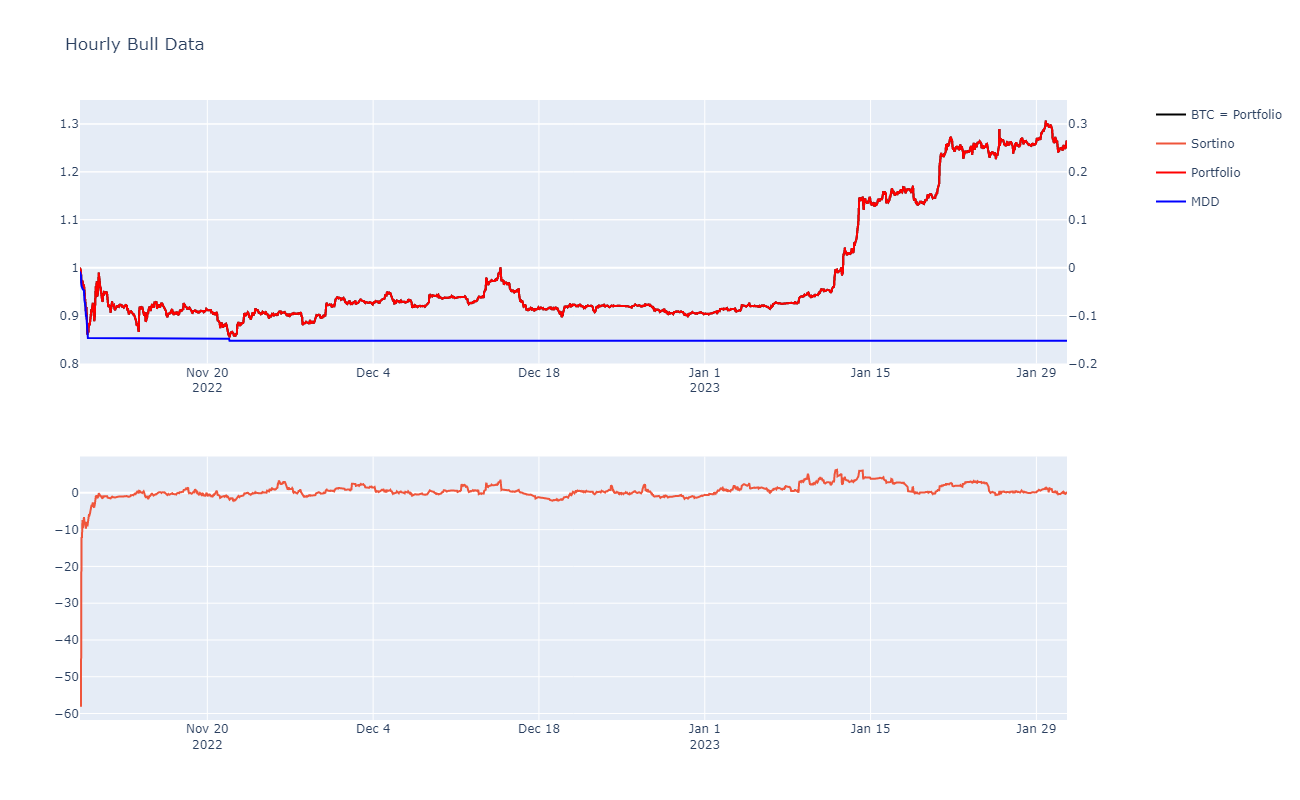
\includegraphics[width=0.94\textwidth]{graphics/results/01_hourly_bull.png}
    \caption{Buy-and-hold metrics for hourly bull data}
    \label{gr:bih:hbu}
\end{figure}

\begin{figure}[H]
    \centering
    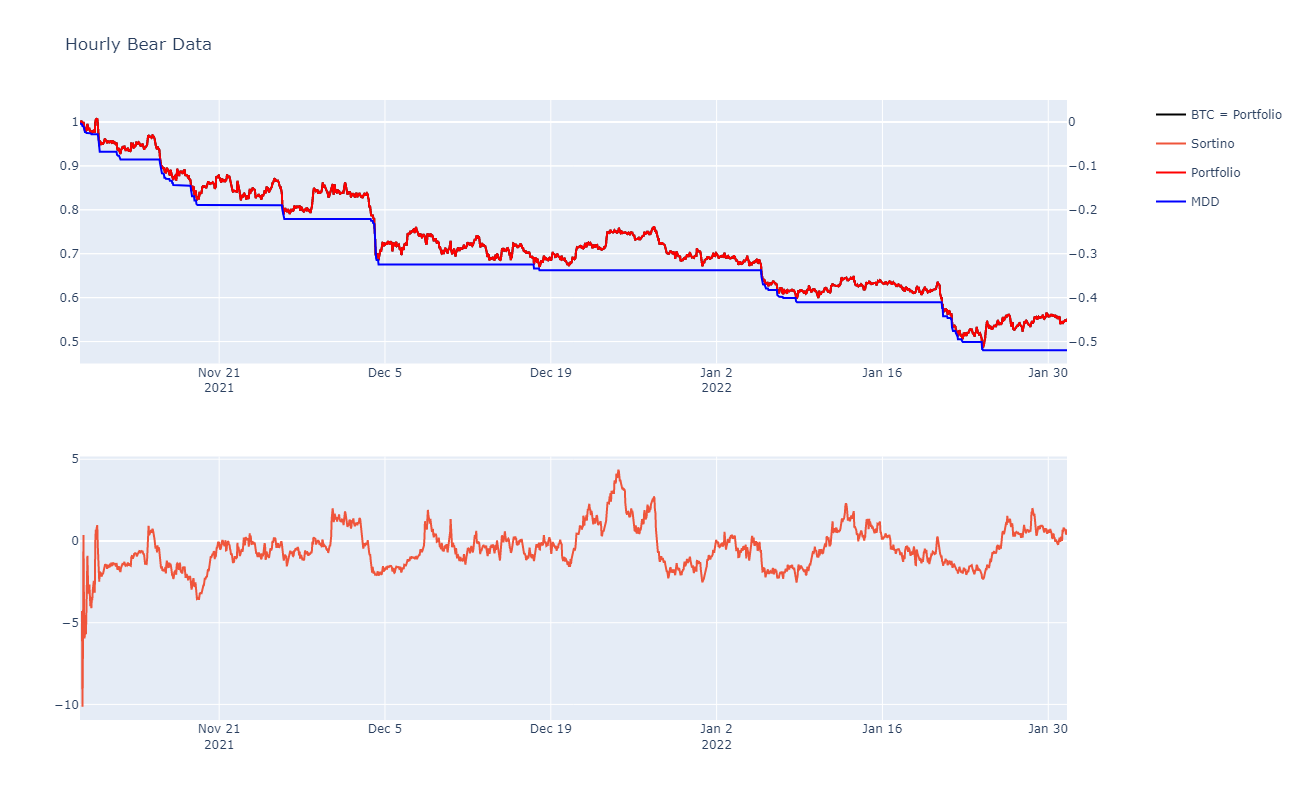
\includegraphics[width=0.94\textwidth]{graphics/results/01_hourly_bear.png}
    \caption{Buy-and-hold metrics for hourly bear data}
    \label{gr:bih:HBr}
\end{figure}

\begin{figure}[H]
    \centering
    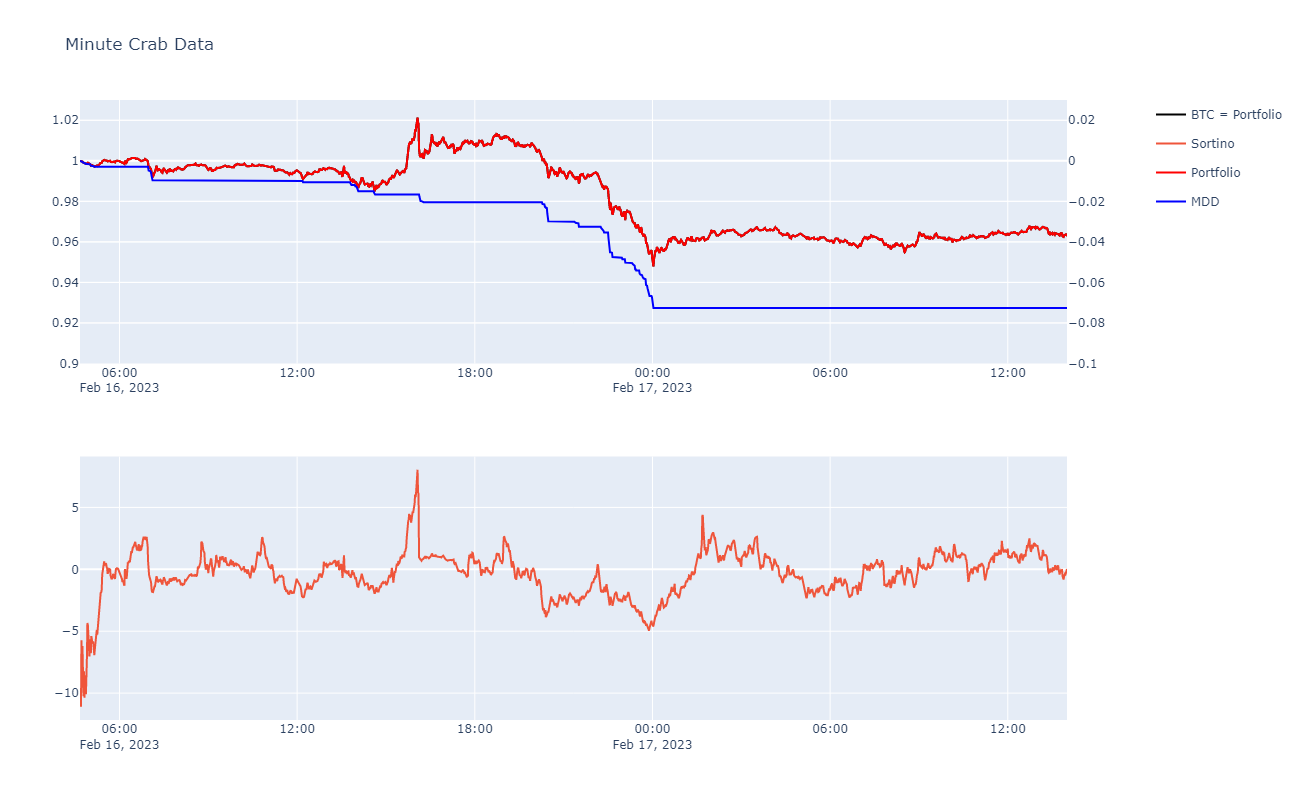
\includegraphics[width=0.94\textwidth]{graphics/results/01_minute_crab.png}
    \caption{Buy-and-hold metrics for minute crab data}
    \label{gr:bih:mcr}
\end{figure}

\begin{figure}[H]
    \centering
    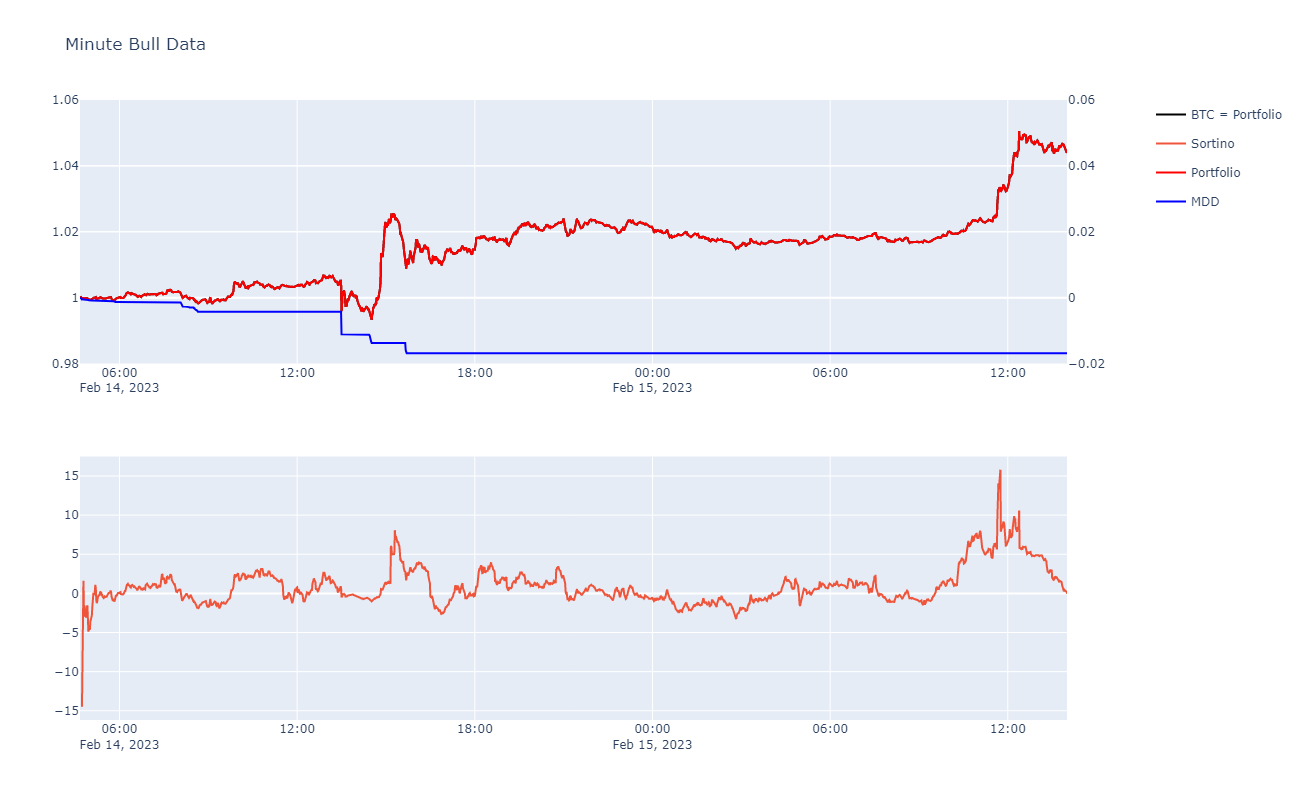
\includegraphics[width=0.94\textwidth]{graphics/results/01_minute_bull.png}
    \caption{Buy-and-hold metrics for minute bull data}
    \label{gr:bih:mbu}
\end{figure}

\subsection{MACD Strategy Agent}
The MACD strategy agent's performance statistics are shown in Table \ref{tab:res-macd}. Since this agent is not a learning agent, the values of $s$, $\tau$, and $\iota$ remain undefined.

Observe that this agent dampens the drawdown and loss in downtrend markets (figs. \ref{gr:macd:HBr}, \ref{gr:macd:mcr}), yet it also limits the profits for some cases and some periods in bull markets (figs. \ref{gr:macd:hbu}, \ref{gr:macd:mbu}). Moreover, MACD strategy shows that it can reduce MDD in all four cases. As for MACD strategy's Sortino ratio, it performs better than benchmark in bear markets, but never in bull or crab markets.

\begin{longtable}[c]{|l|r|r|r|c|c|c|l|}
\caption{MACD strategy agent statistics}
\label{tab:res-macd}\\
\hline
\multicolumn{1}{|c|}{} & \multicolumn{1}{c|}{\textbf{Return}} & \multicolumn{1}{c|}{\textbf{MDD}} & \multicolumn{1}{c|}{\textbf{Sortino}} &
\multicolumn{1}{c|}{\textbf{$\overline{\Delta\phi_{MACD,\odot}}$}} & \textbf{\textit{$s$}} & \multicolumn{1}{c|}{\textbf{Figure}} \\ \hline
\endfirsthead
%
\multicolumn{7}{c}%
{{\bfseries Table \thetable\ continued from previous page}} \\
\endhead
%
\textbf{\texttt{HBu}} & 0.2161 & 0.1159 & 0.0421 & 0.0620 & - &  \ref{gr:macd:hbu} \\ \hline
\textbf{\texttt{HBr}} & -0.3389 & 0.3570 & 0.6351 & 0.1363 & - &  \ref{gr:macd:HBr} \\ \hline
\textbf{\texttt{MCr}} & -0.0148 & 0.0427 & 0.4893 & 0.0118 & - &  \ref{gr:macd:mcr} \\ \hline
\textbf{\texttt{MBu}} & 0.0364 & 0.0124 & -0.1592 & -0.0008 & - &  \ref{gr:macd:mbu} \\ \hline
\end{longtable}

Figures \ref{gr:macd:HBr}, \ref{gr:macd:hbu}, \ref{gr:macd:mcr}, and \ref{gr:macd:mbu} show the full per-timeframe statistics of the recorded metrics. The upper part of the graphs shows three lines: (1) Black line: BTC closing price of each timeframe relative to the closing price of the first timeframe, (2) Red line: portfolio value of each timeframe relative to the initial investment, (3) Blue line: maximum drawdown of the portfolio. The lower part of the graphs contains two information: (1) Green line: 100-timeframe Sortino ratio of each timeframe, (2) Bar chart: shows the value of \texttt{macd\_histo} at each timeframe.

\begin{figure}[H]
    \centering
    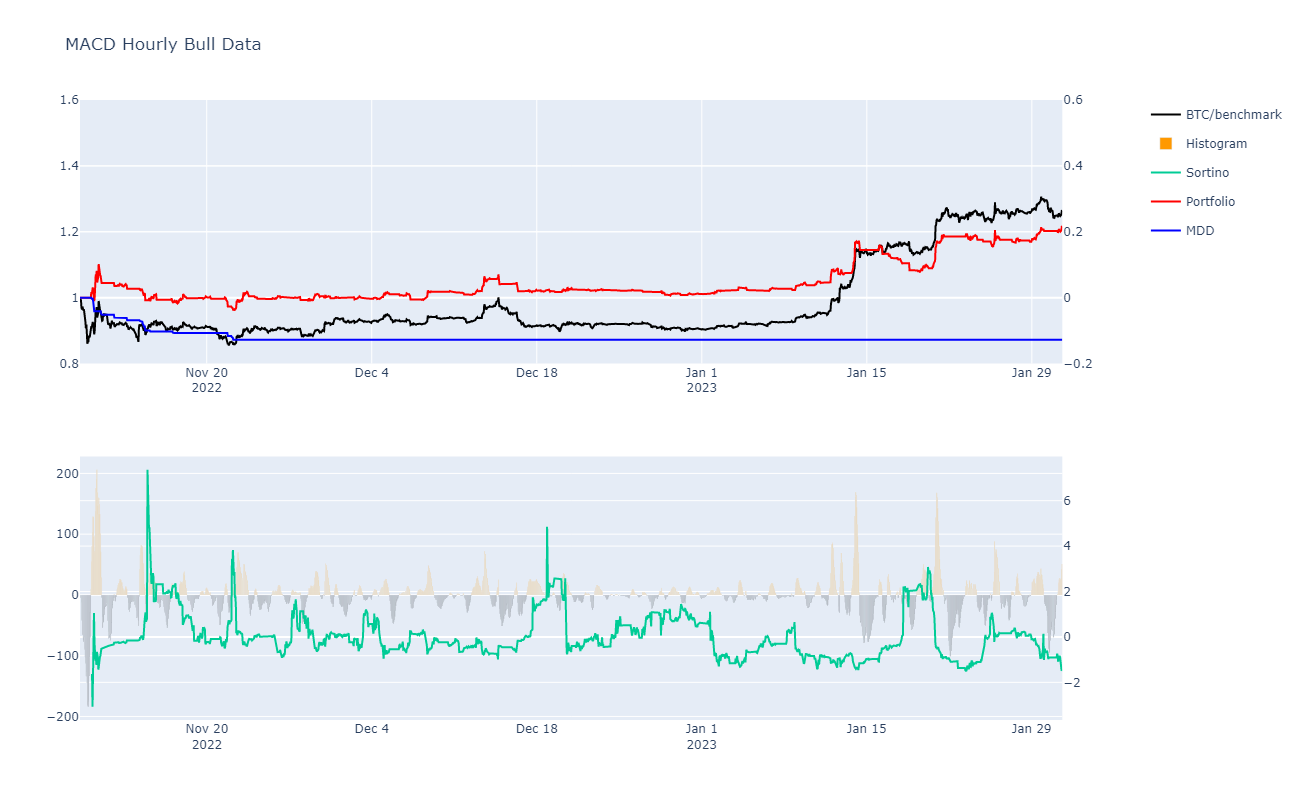
\includegraphics[width=0.94\textwidth]{graphics/results/02_macd_hourly_bull.png}
    \caption{MACD strategy metrics for hourly bull data}
    \label{gr:macd:hbu}
\end{figure}

\begin{figure}[H]
    \centering
    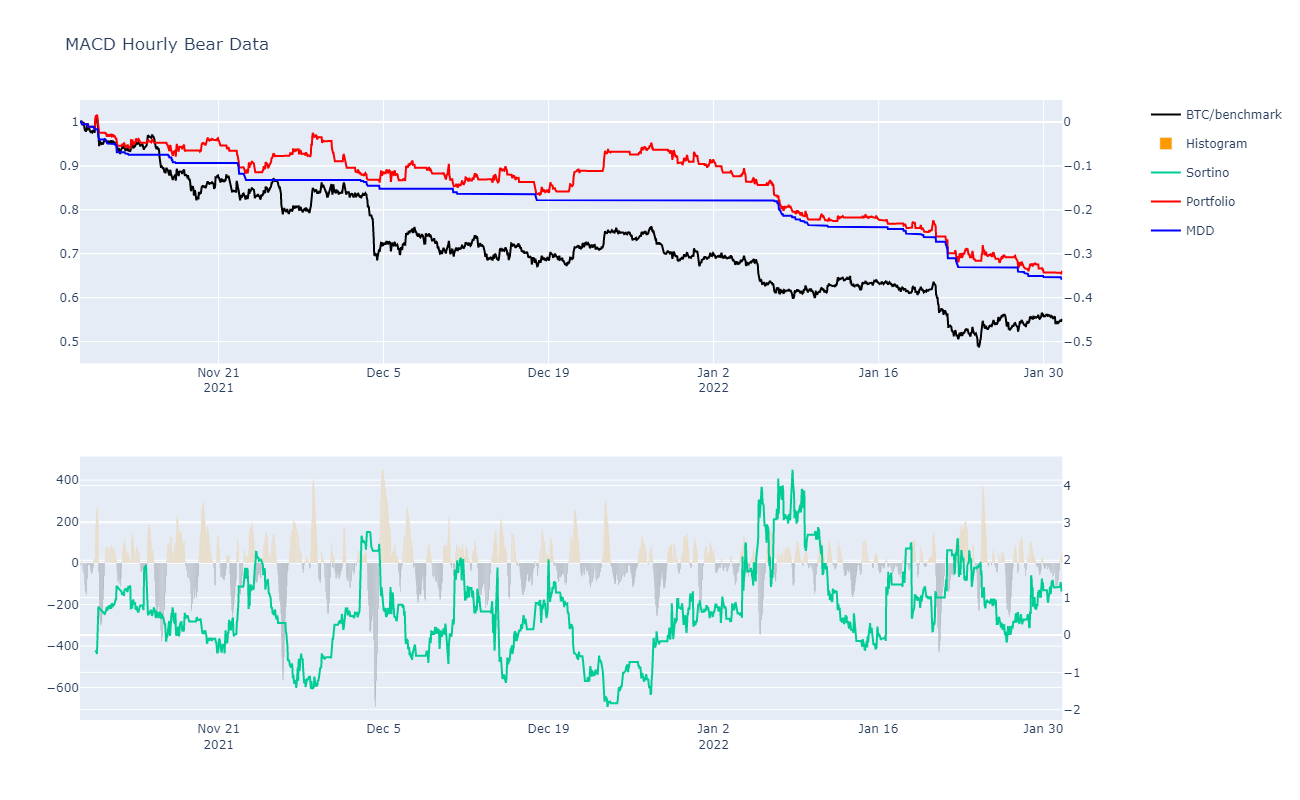
\includegraphics[width=0.94\textwidth]{graphics/results/02_macd_hourly_bear.png}
    \caption{MACD strategy metrics for hourly bear data}
    \label{gr:macd:HBr}
\end{figure}

\begin{figure}[H]
    \centering
    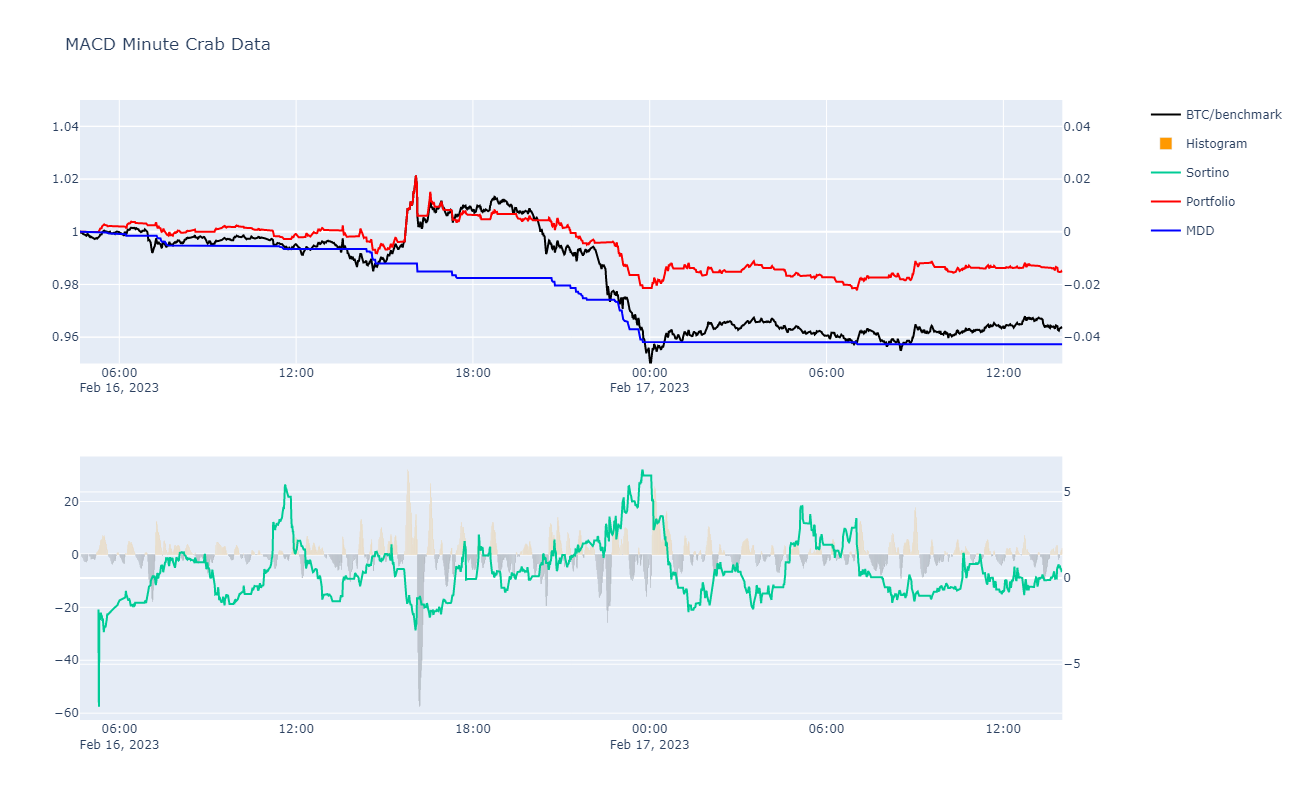
\includegraphics[width=0.94\textwidth]{graphics/results/02_macd_minute_crab.png}
    \caption{MACD strategy metrics for minute crab data}
    \label{gr:macd:mcr}
\end{figure}

\begin{figure}[H]
    \centering
    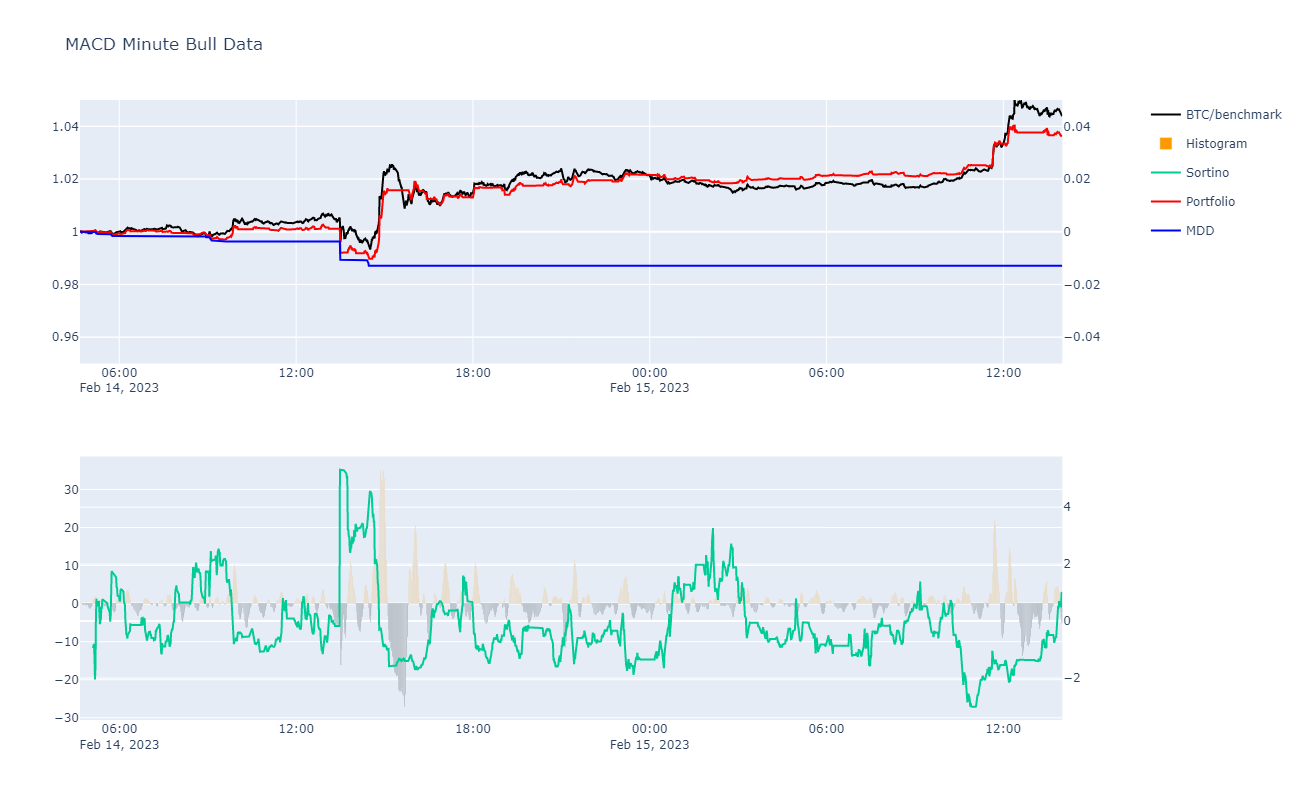
\includegraphics[width=0.94\textwidth]{graphics/results/02_macd_minute_bull.png}
    \caption{MACD strategy metrics for minute bull data}
    \label{gr:macd:mbu}
\end{figure}

\subsection{DQN Strategy Agent (Discrete)}
The DQN agent is the first RL agent to be presented in this chapter, operating in the discrete action space. Using training data (see Fig. \ref{gr:dqn:train}), the agent performs best only at early timestamps (between 100,000 to 500,000 timesteps $\approx$ 9 to 45 episodes). After around $s=$ 768,936 timestamps or 69 episodes ($\sim$2,500 seconds of training), the rewards and return value flatten.

\begin{figure}[H]
    \centering
    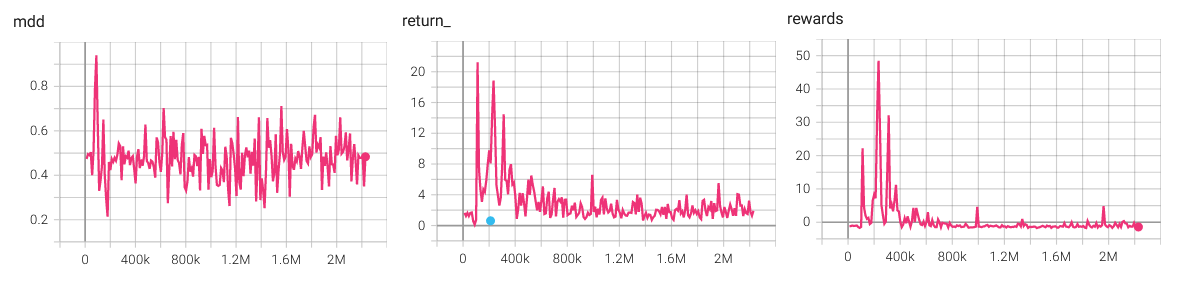
\includegraphics[width=0.99\textwidth]{graphics/trainphoto/dqntrain.png}
    \caption{DQN Training Results}
    \label{gr:dqn:train}
\end{figure}

DQN Agent's test results are given in Table \ref{resl:dqn}. By the average portfolio value over benchmark, the DQN agent outperforms the benchmark in all cases, while it fails to give the highest final value for \texttt{HBu} and \texttt{MBu} test datasets. The DQN agent, however, produces lower MDD which signifies that this agent is more risk-averse than the buy-and-hold agent.

\begin{longtable}[c]{|l|rrr|rrr|r|c|}
\caption{DQN Test Results}
\label{resl:cont-dqn}\\
\hline
\multicolumn{1}{|c|}{\multirow{2}{*}{\textbf{$\mathcal{D}$}}} & \multicolumn{3}{c|}{\textbf{Agent}} & \multicolumn{3}{c|}{\textbf{Benchmark}} & \multicolumn{1}{c|}{\multirow{2}{*}{\textbf{$\overline{\Delta\phi_{\alpha,\odot}}$}}} & \multirow{2}{*}{\textbf{Fig.}} \\ \cline{2-7}
\multicolumn{1}{|c|}{} & \multicolumn{1}{c|}{\textbf{Return}} & \multicolumn{1}{c|}{\textbf{MDD}} & \multicolumn{1}{c|}{\textit{\textbf{Sortino}}} & \multicolumn{1}{c|}{\textbf{Return}} & \multicolumn{1}{c|}{\textbf{MDD}} & \multicolumn{1}{c|}{\textit{\textbf{Sortino}}} & \multicolumn{1}{c|}{} &  \\ \hline
\endfirsthead
%
\multicolumn{9}{c}%
{{\bfseries Table \thetable\ continued from previous page}} \\
\endhead
%
\textbf{\texttt{HBu}} & \multicolumn{1}{r|}{0.1540} & \multicolumn{1}{r|}{0.1812} & \textit{-0.2212} & \multicolumn{1}{r|}{\textbf{0.2643}} & \multicolumn{1}{r|}{\textbf{0.1174}} & \textit{0.7060} & 0.0204 & \ref{f-dqn-hbu} \\ \hline
\textbf{\texttt{HBr}} & \multicolumn{1}{r|}{\textbf{-0.1184}} & \multicolumn{1}{r|}{\textbf{0.1343}} & \textit{0.7485} & \multicolumn{1}{r|}{-0.4484} & \multicolumn{1}{r|}{0.5199} & \textit{-0.3982} & 0.3015 & \ref{f-dqn-hbr} \\ \hline
\textbf{\texttt{MCr}} & \multicolumn{1}{r|}{\textbf{0.0296}} & \multicolumn{1}{r|}{\textbf{0.0313}} & \textit{1.1557} & \multicolumn{1}{r|}{-0.0361} & \multicolumn{1}{r|}{0.0725} & \textit{-0.2276} & 0.0383 & \ref{f-dqn-mcr} \\ \hline
\textbf{\texttt{MBu}} & \multicolumn{1}{r|}{0.0357} & \multicolumn{1}{r|}{\textbf{0.0061}} & \textit{-0.3521} & \multicolumn{1}{r|}{\textbf{0.0441}} & \multicolumn{1}{r|}{0.0164} & \textit{1.0024} & 0.0102 & \ref{f-dqn-mbu} \\ \hline
\end{longtable}

\begin{figure}[H]
    \centering
    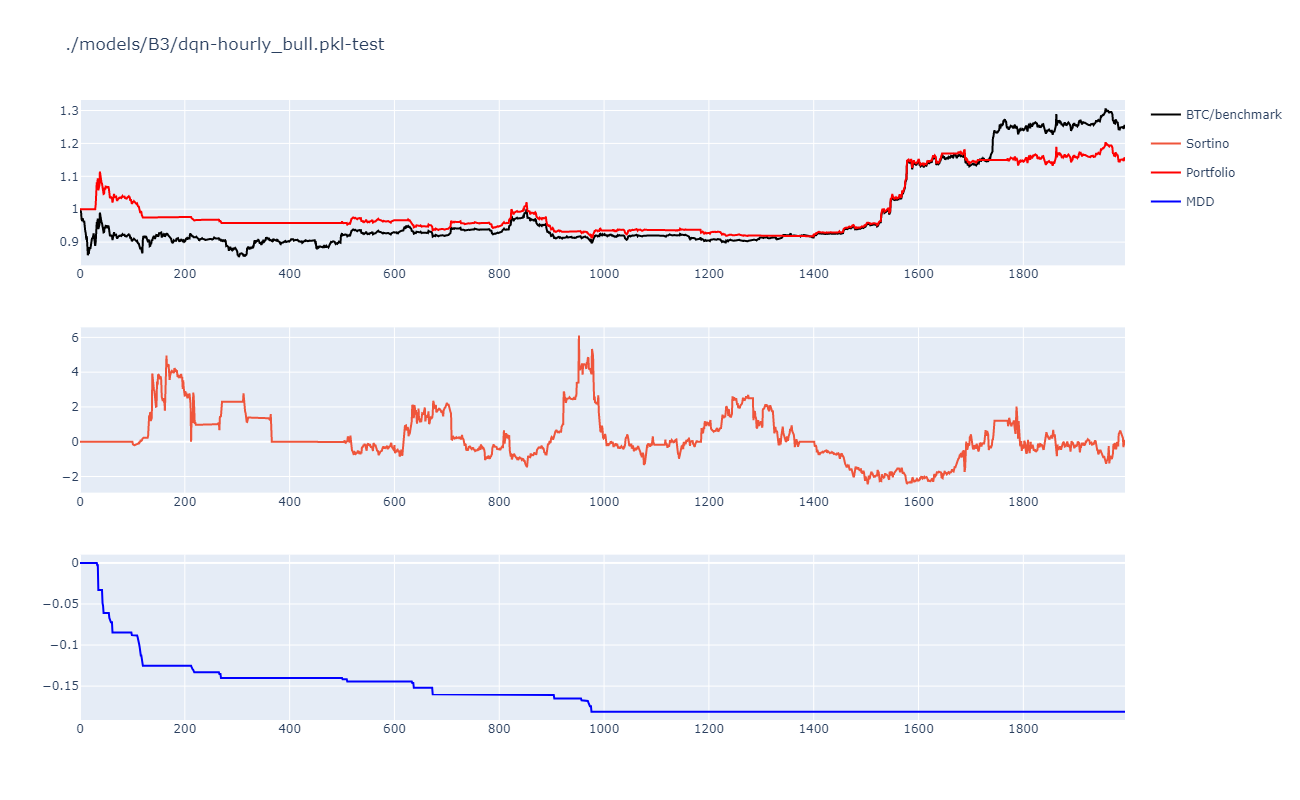
\includegraphics[width=0.94\textwidth]{graphics/testphoto/dqn-hbu.png}
    \caption{DQN agent metrics for hourly bull data}
    \label{f-dqn-hbu}
\end{figure}

\begin{figure}[H]
    \centering
    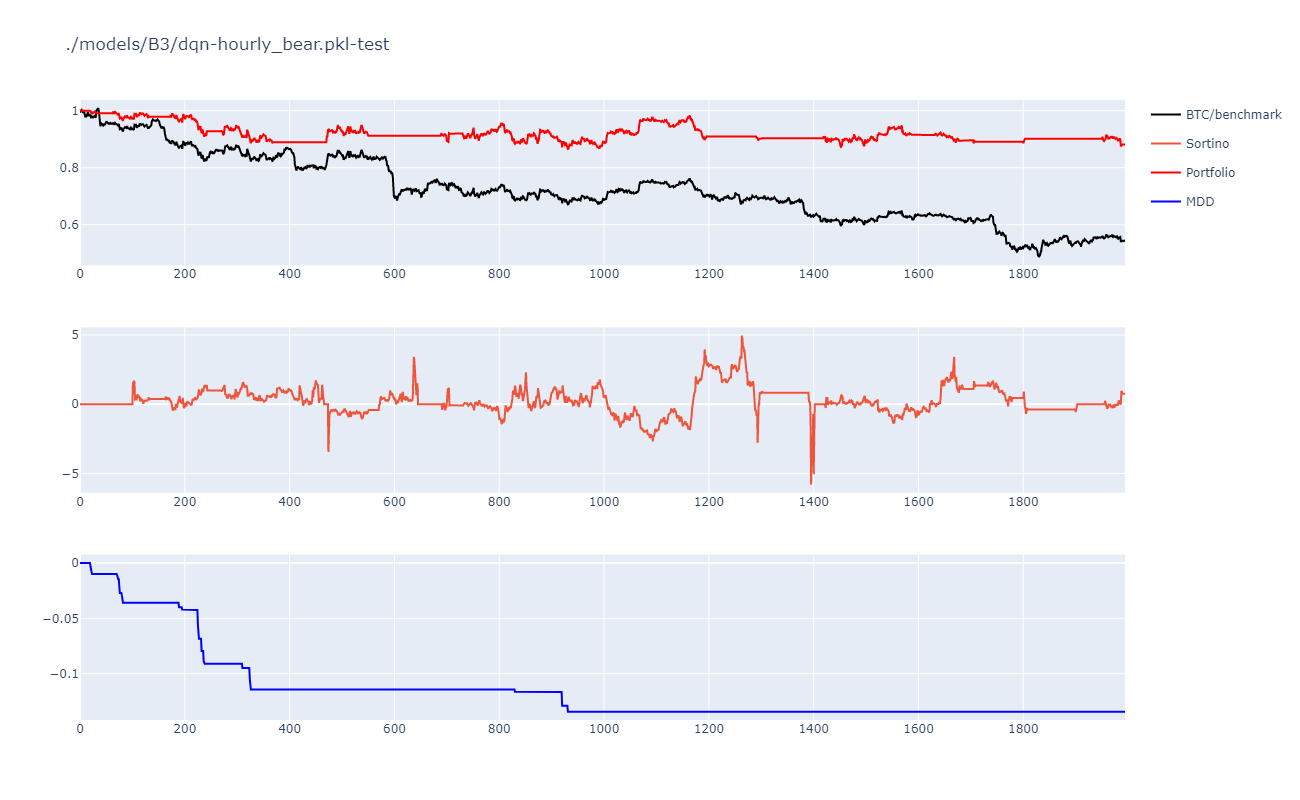
\includegraphics[width=0.94\textwidth]{graphics/testphoto/dqn-hbr.png}
    \caption{DQN agent metrics for hourly bear data}
    \label{f-dqn-hbr}
\end{figure}

\begin{figure}[H]
    \centering
    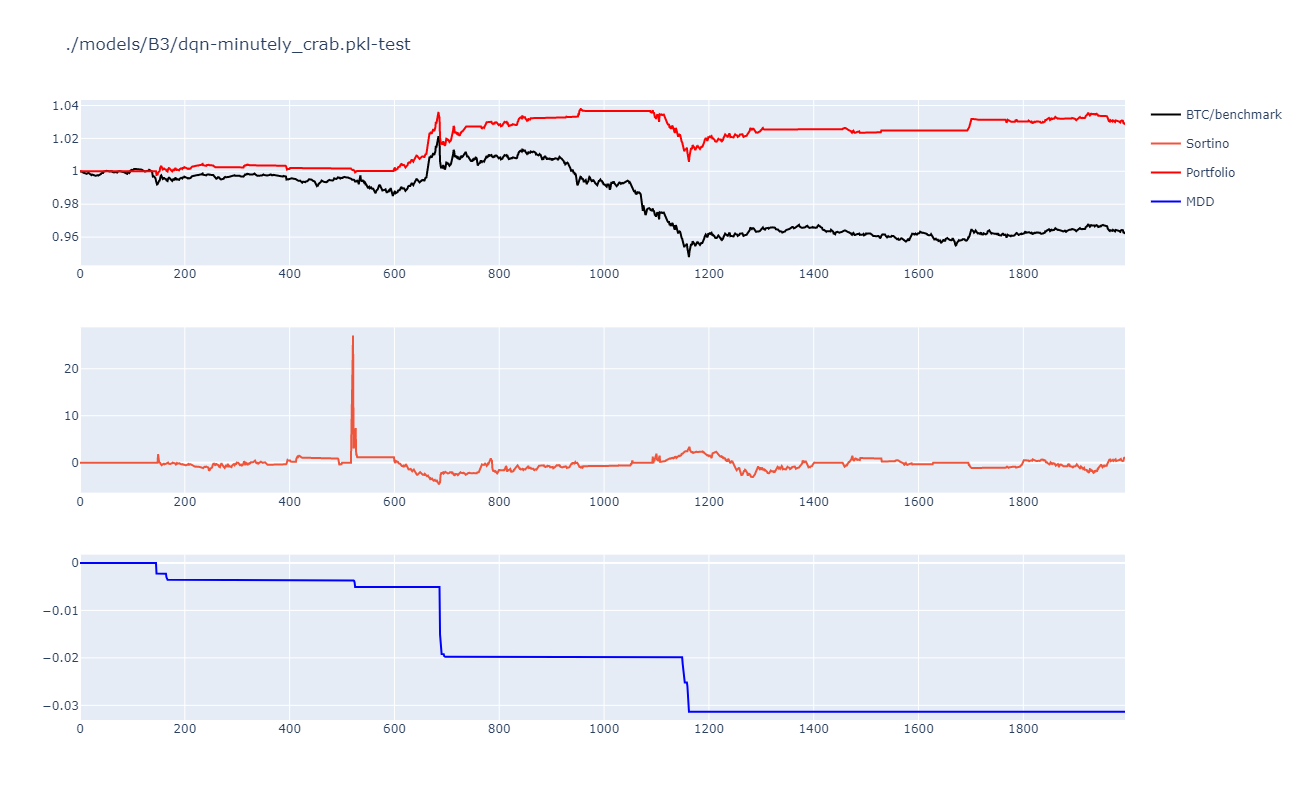
\includegraphics[width=0.94\textwidth]{graphics/testphoto/dqn-mcr.png}
    \caption{DQN agent metrics for minute crab data}
    \label{f-dqn-mcr}
\end{figure}

\begin{figure}[H]
    \centering
    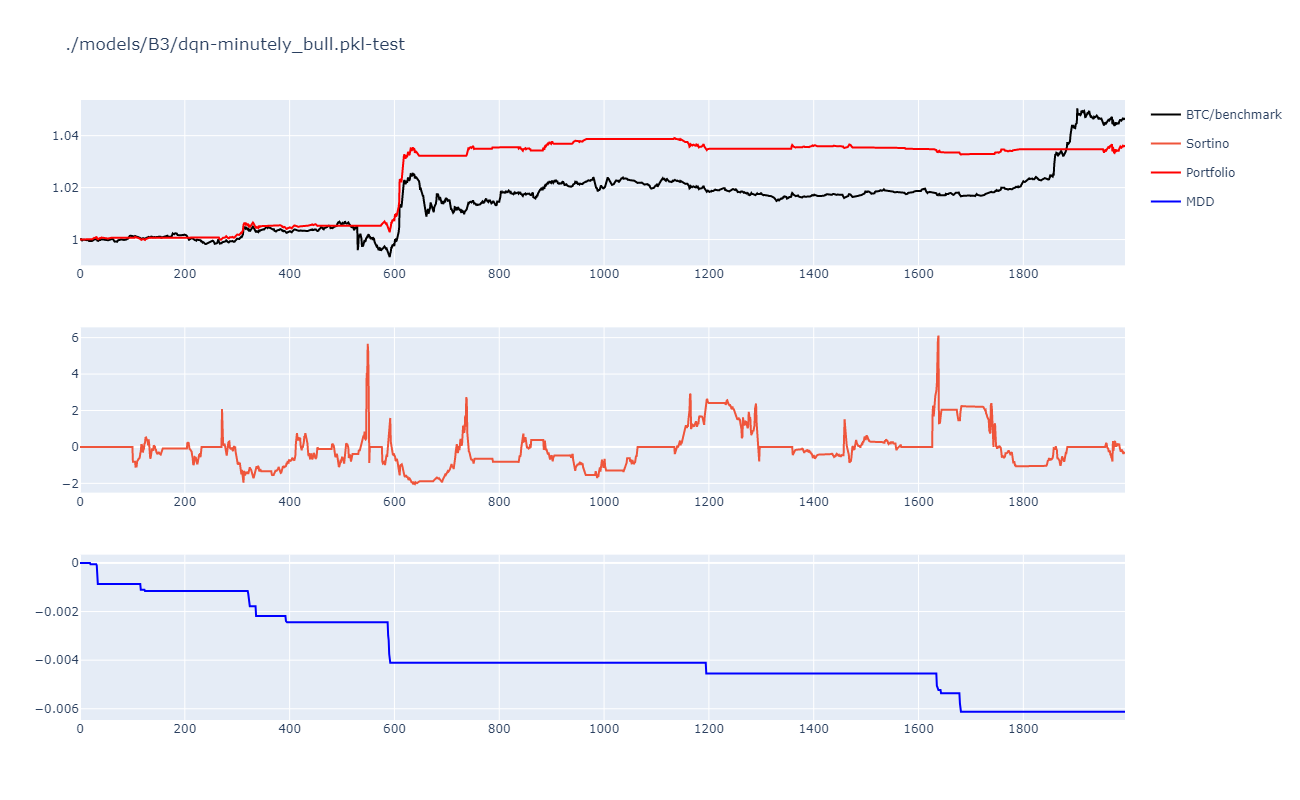
\includegraphics[width=0.94\textwidth]{graphics/testphoto/dqn-mbu.png}
    \caption{DQN agent metrics for minute bull data}
    \label{f-dqn-mbu}
\end{figure}

\subsection{A2C Strategy Agent (Discrete)}
This A2C agent is used with a discrete action space. Using training data (see Fig. \ref{gr:a2cd:train}), the agent, by all factors, converges quickly at around $\sim$45,000 timesteps (4 episodes, $\sim$90 seconds of training). After that, there is virtually no improvement nor deterioration of the model.

\begin{figure}[H]
    \centering
    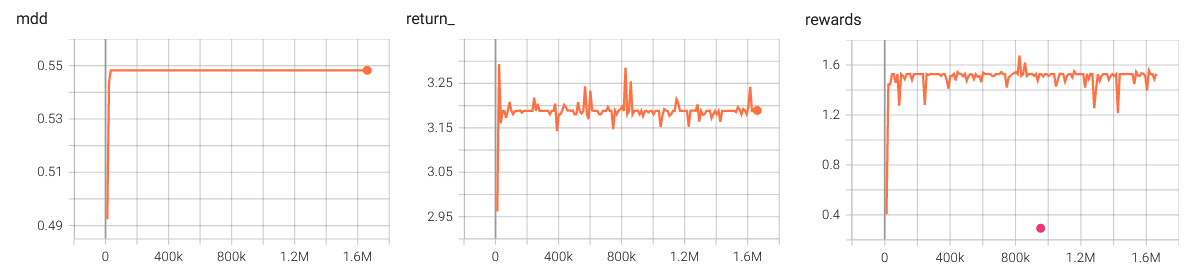
\includegraphics[width=0.99\textwidth]{graphics/trainphoto/a2cd-train.png}
    \caption{Discrete A2C Training Results}
    \label{gr:a2cd:train}
\end{figure}

Despite the quick stable model turnout, it is suspected that the model only performs a minimal number of trades and just holds the one-time bought until the end, rendering it to be exactly comparable with the buy-and-hold agent. Refer to Table \ref{resl:disc-a2c}'s $\overline{\Delta\phi_{\alpha,\odot}}$ column which shows that the average difference between the portfolio values of this agent and the benchmark agent is less than 0.5 percent in all cases.

\begin{longtable}[c]{|l|rrr|rrr|r|c|}
\caption{Discrete A2C Test Results}
\label{resl:disc-a2c}\\
\hline
\multicolumn{1}{|c|}{\multirow{2}{*}{\textbf{$\mathcal{D}$}}} & \multicolumn{3}{c|}{\textbf{Agent}} & \multicolumn{3}{c|}{\textbf{Benchmark}} & \multicolumn{1}{c|}{\multirow{2}{*}{\textbf{$\overline{\Delta\phi_{\alpha,\odot}}$}}} & \multirow{2}{*}{\textbf{Fig.}} \\ \cline{2-7}
\multicolumn{1}{|c|}{} & \multicolumn{1}{c|}{\textbf{Return}} & \multicolumn{1}{c|}{\textbf{MDD}} & \multicolumn{1}{c|}{\textit{\textbf{Sortino}}} & \multicolumn{1}{c|}{\textbf{Return}} & \multicolumn{1}{c|}{\textbf{MDD}} & \multicolumn{1}{c|}{\textit{\textbf{Sortino}}} & \multicolumn{1}{c|}{} &  \\ \hline
\endfirsthead
%
\multicolumn{9}{c}%
{{\bfseries Table \thetable\ continued from previous page}} \\
\endhead
%
\textbf{\texttt{HBu}} & \multicolumn{1}{r|}{0.2568} & \multicolumn{1}{r|}{0.1425} & \textit{-0.2843} & \multicolumn{1}{r|}{\textbf{0.2643}} & \multicolumn{1}{r|}{\textbf{0.1174}} & \textit{0.7060} & 0.0035 & \ref{f-a2c-cont-hbu} \\ \hline
\textbf{\texttt{HBr}} & \multicolumn{1}{r|}{-0.4543} & \multicolumn{1}{r|}{\textbf{0.5174}} & \textit{-0.7186} & \multicolumn{1}{r|}{\textbf{-0.4484}} & \multicolumn{1}{r|}{0.5199} & \textit{-0.3982} & -0.0009 & \ref{f-a2c-cont-hbr} \\ \hline
\textbf{\texttt{MCr}} & \multicolumn{1}{r|}{-0.0368} & \multicolumn{1}{r|}{\textbf{0.0719}} & \textit{0.8994} & \multicolumn{1}{r|}{\textbf{-0.0361}} & \multicolumn{1}{r|}{0.0725} & \textit{-0.2276} & 0.0000 & \ref{f-a2c-cont-mcr} \\ \hline
\textbf{\texttt{MBu}} & \multicolumn{1}{r|}{\textbf{0.0462}} & \multicolumn{1}{r|}{0.0165} & \textit{-0.3752} & \multicolumn{1}{r|}{0.0441} & \multicolumn{1}{r|}{\textbf{0.0164}} & \textit{1.0024} & 0.0000 & \ref{f-a2c-cont-mbu} \\ \hline
\end{longtable}

\begin{figure}[H]
    \centering
    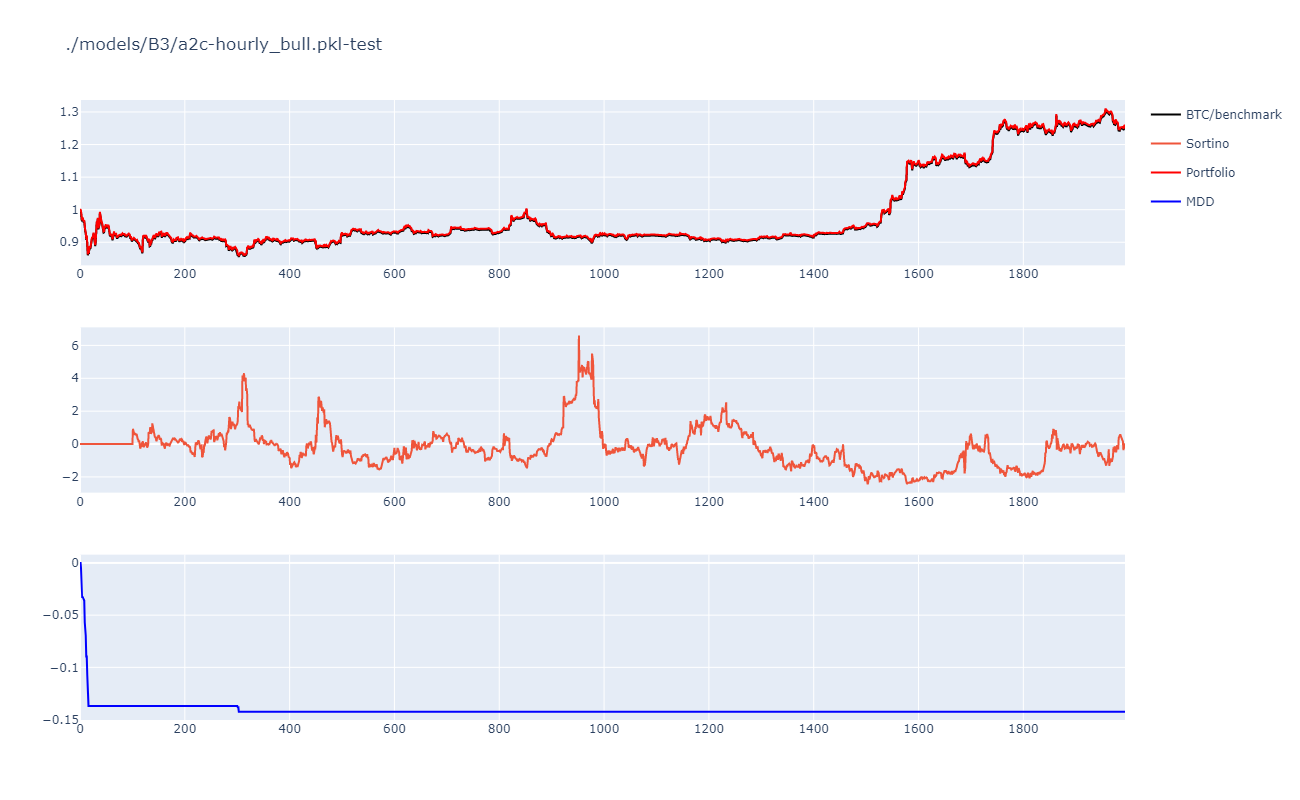
\includegraphics[width=0.94\textwidth]{graphics/testphoto/a2c-disc-hbu.png}
    \caption{Discrete A2C agent metrics for hourly bull data}
    \label{f-a2c-disc-hbu}
\end{figure}

\begin{figure}[H]
    \centering
    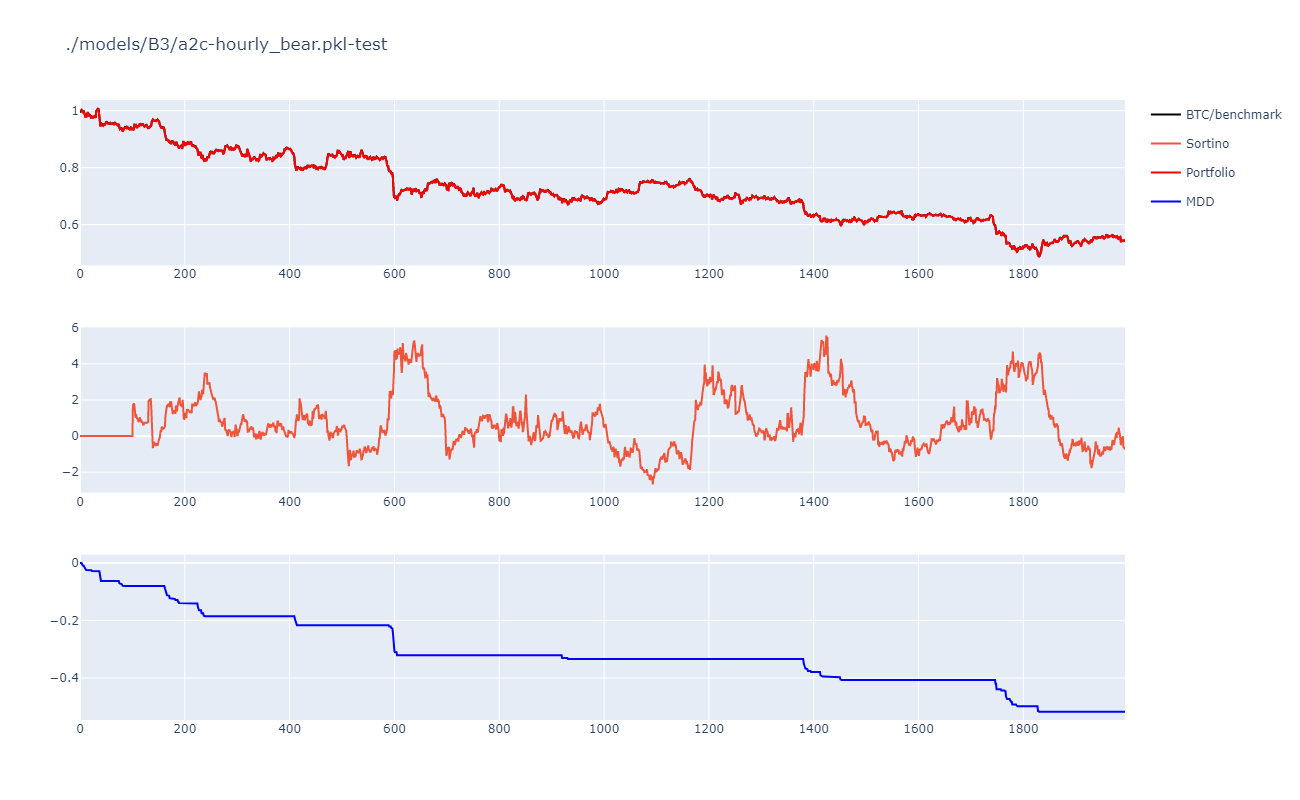
\includegraphics[width=0.94\textwidth]{graphics/testphoto/a2c-disc-hbr.png}
    \caption{Discrete A2C agent metrics for hourly bear data}
    \label{f-a2c-disc-hbr}
\end{figure}

\begin{figure}[H]
    \centering
    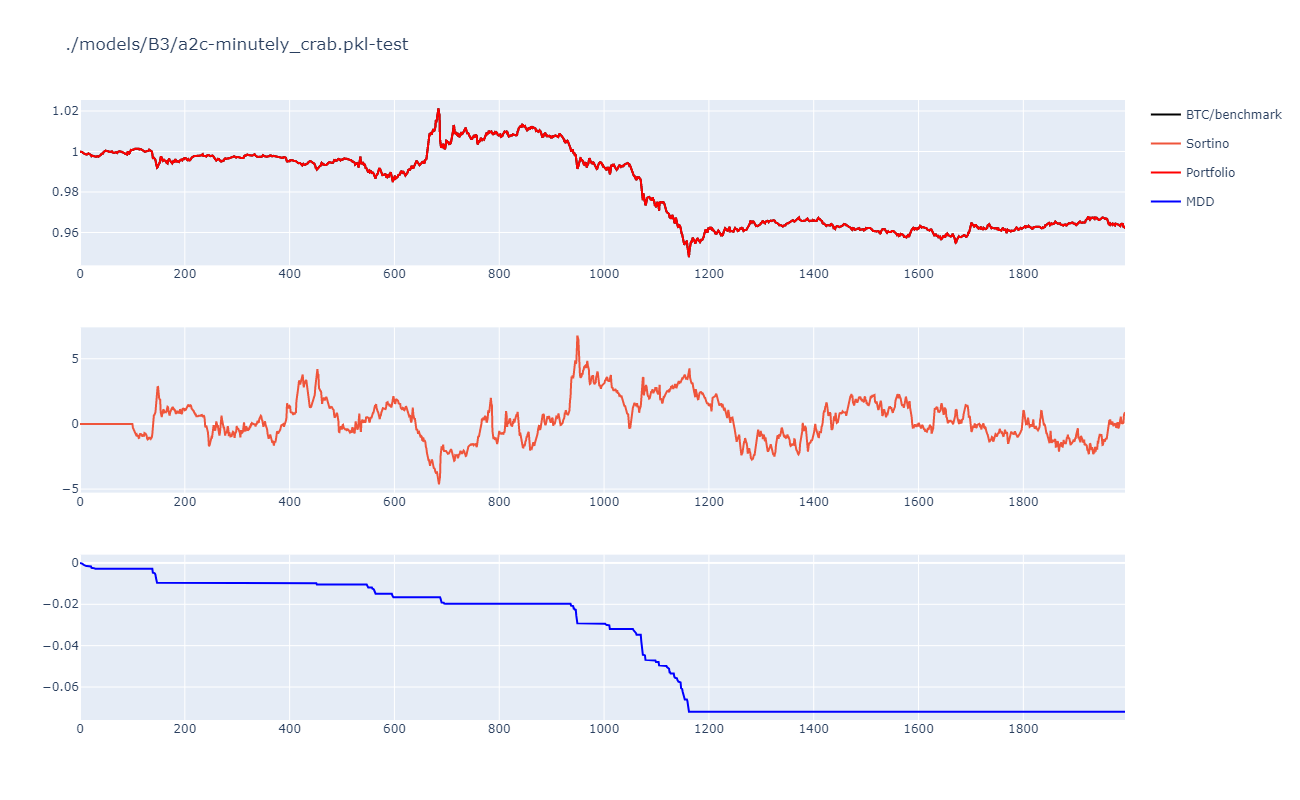
\includegraphics[width=0.94\textwidth]{graphics/testphoto/a2c-disc-mcr.png}
    \caption{Discrete A2C agent metrics for minute crab data}
    \label{f-a2c-disc-mcr}
\end{figure}

\begin{figure}[H]
    \centering
    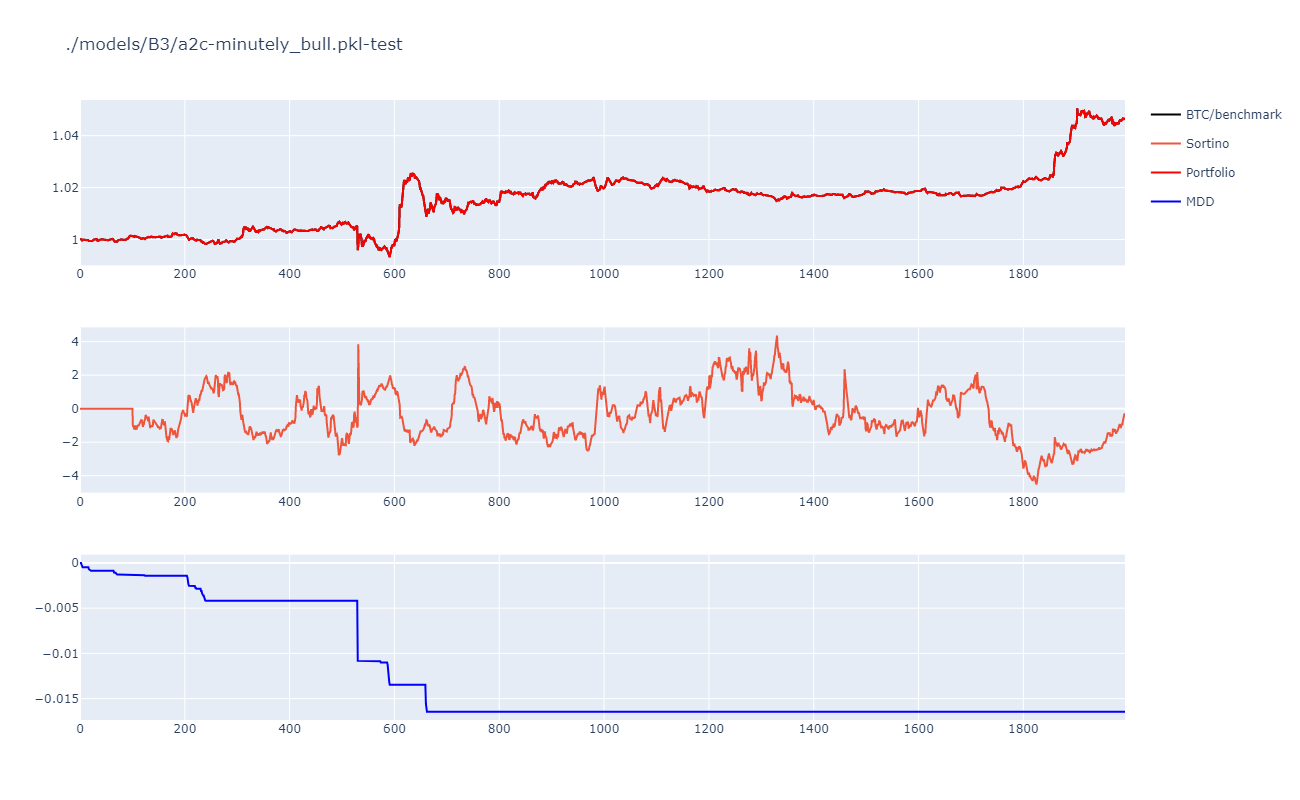
\includegraphics[width=0.94\textwidth]{graphics/testphoto/a2c-disc-mbu.png}
    \caption{Discrete A2C agent metrics for minute bull data}
    \label{f-a2c-disc-mbu}
\end{figure}

\subsection{A2C Strategy Agent (Continuous)}
This A2C agent is used with a continuous action space. Using training data (see Fig. \ref{gr:a2cd:train}), the agent never finds a stable ground even after more than 1,671,600 timestamps (150 episodes, 5,500 seconds): the total reward and return still fluctuates randomly, unlike its discrete counterpart. The models with zero reward did not generate any trade, including the final model, hence the last non-zero-reward model at timestamp 1,348,424 (121st episode) is taken as its representative model.

\begin{figure}[H]
    \centering
    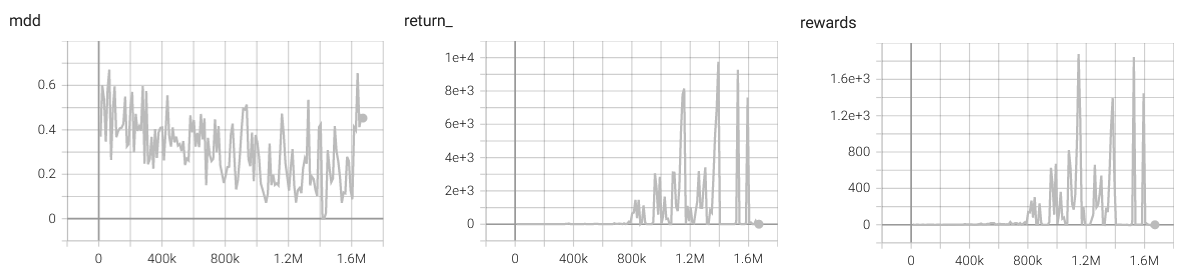
\includegraphics[width=0.99\textwidth]{graphics/trainphoto/a2cc-train.png}
    \caption{Continuous A2C Training Results}
    \label{gr:a2cc:train}
\end{figure}

Compared to the benchmark, the representative Continuous A2C model results in a slightly more satisfiable performance in minute test datasets, at 1.68\% (crab) and 0.23\% (bull) average portfolio differences, 40\% less drawdown, and higher final return. Conversely, this model fails to produce better performance than benchmark in all aspects. See Table \ref{resl:cont-a2c}.

\begin{longtable}[c]{|l|rrr|rrr|r|c|}
\caption{Continuous A2C Test Results}
\label{resl:cont-a2c}\\
\hline
\multicolumn{1}{|c|}{\multirow{2}{*}{\textbf{$\mathcal{D}$}}} & \multicolumn{3}{c|}{\textbf{Agent}} & \multicolumn{3}{c|}{\textbf{Benchmark}} & \multicolumn{1}{c|}{\multirow{2}{*}{\textbf{$\overline{\Delta\phi_{\alpha,\odot}}$}}} & \multirow{2}{*}{\textbf{Fig.}} \\ \cline{2-7}
\multicolumn{1}{|c|}{} & \multicolumn{1}{c|}{\textbf{Return}} & \multicolumn{1}{c|}{\textbf{MDD}} & \multicolumn{1}{c|}{\textit{\textbf{Sortino}}} & \multicolumn{1}{c|}{\textbf{Return}} & \multicolumn{1}{c|}{\textbf{MDD}} & \multicolumn{1}{c|}{\textit{\textbf{Sortino}}} & \multicolumn{1}{c|}{} &  \\ \hline
\endfirsthead
%
\multicolumn{9}{c}%
{{\bfseries Table \thetable\ continued from previous page}} \\
\endhead
%
\textbf{\texttt{HBu}} & \multicolumn{1}{r|}{0.0060} & \multicolumn{1}{r|}{0.1622} & \textit{-0.5541} & \multicolumn{1}{r|}{\textbf{0.2643}} & \multicolumn{1}{r|}{\textbf{0.1174}} & \textit{0.7060} & -0.0602 & \ref{f-a2c-disc-hbu} \\ \hline
\textbf{\texttt{HBr}} & \multicolumn{1}{r|}{-0.4824} & \multicolumn{1}{r|}{0.5618} & \textit{-1.6495} & \multicolumn{1}{r|}{\textbf{-0.4484}} & \multicolumn{1}{r|}{\textbf{0.5199}} & \textit{-0.3982} & -0.0320 & \ref{f-a2c-disc-hbr} \\ \hline
\textbf{\texttt{MCr}} & \multicolumn{1}{r|}{\textbf{-0.0137}} & \multicolumn{1}{r|}{\textbf{0.0462}} & \textit{0.6625} & \multicolumn{1}{r|}{-0.0361} & \multicolumn{1}{r|}{0.0725} & \textit{-0.2276} & 0.0168 & \ref{f-a2c-disc-mcr} \\ \hline
\textbf{\texttt{MBu}} & \multicolumn{1}{r|}{\textbf{0.0480}} & \multicolumn{1}{r|}{\textbf{0.0101}} & \textit{-1.2651} & \multicolumn{1}{r|}{0.0441} & \multicolumn{1}{r|}{0.0164} & \textit{1.0024} & 0.0023 & \ref{f-a2c-disc-mbu} \\ \hline
\end{longtable}

\begin{figure}[H]
    \centering
    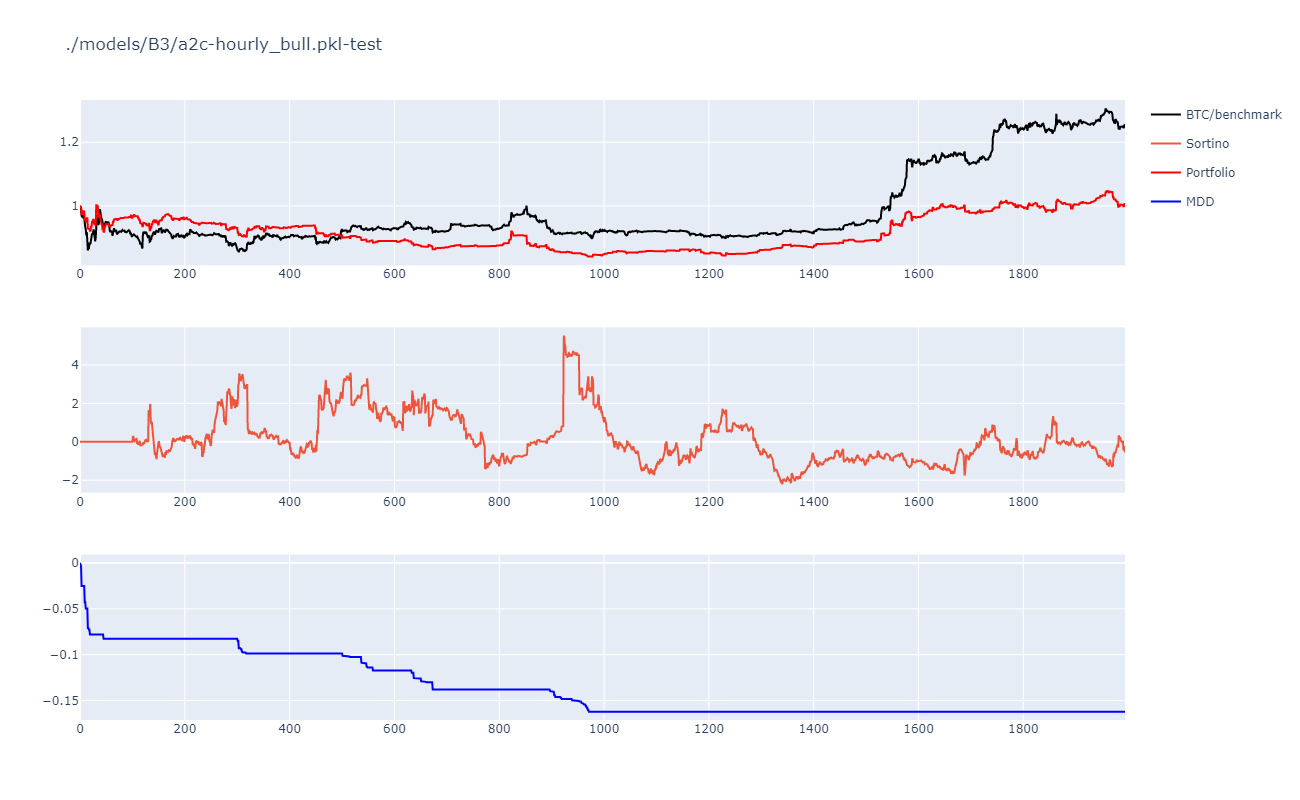
\includegraphics[width=0.94\textwidth]{graphics/testphoto/a2c-cont-hbu.png}
    \caption{Continuous A2C agent metrics for hourly bull data}
    \label{f-a2c-cont-hbu}
\end{figure}

\begin{figure}[H]
    \centering
    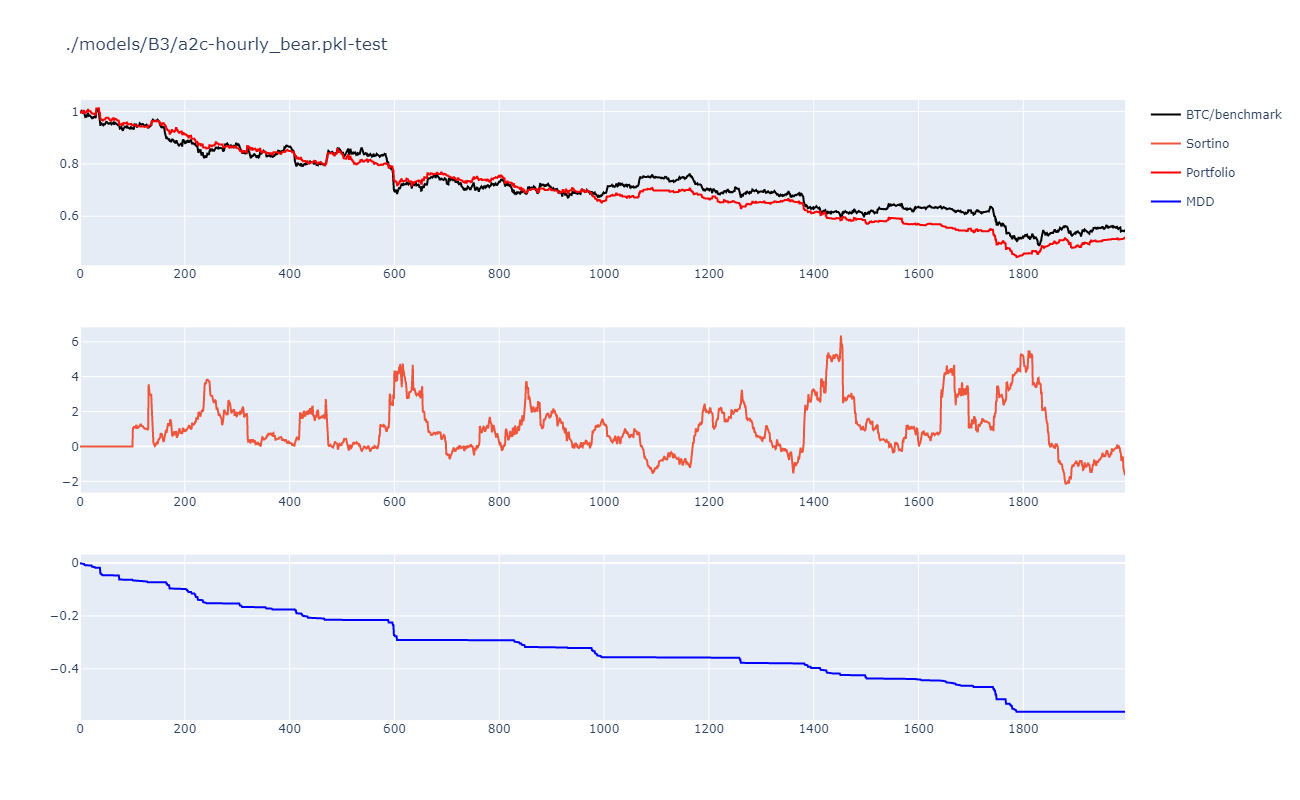
\includegraphics[width=0.94\textwidth]{graphics/testphoto/a2c-cont-hbr.png}
    \caption{Continuous A2C agent metrics for hourly bear data}
    \label{f-a2c-cont-hbr}
\end{figure}

\begin{figure}[H]
    \centering
    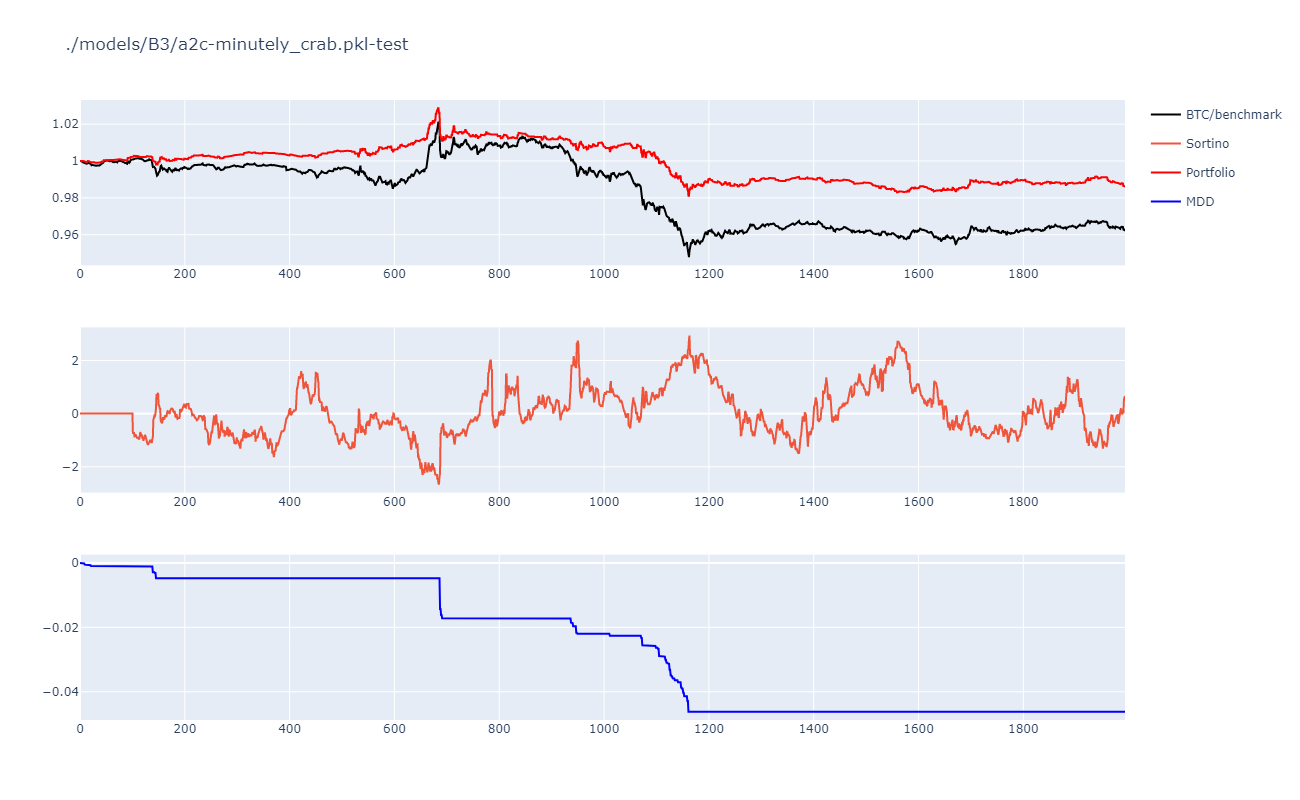
\includegraphics[width=0.94\textwidth]{graphics/testphoto/a2c-cont-mcr.png}
    \caption{Continuous A2C agent metrics for minute crab data}
    \label{f-a2c-cont-mcr}
\end{figure}

\begin{figure}[H]
    \centering
    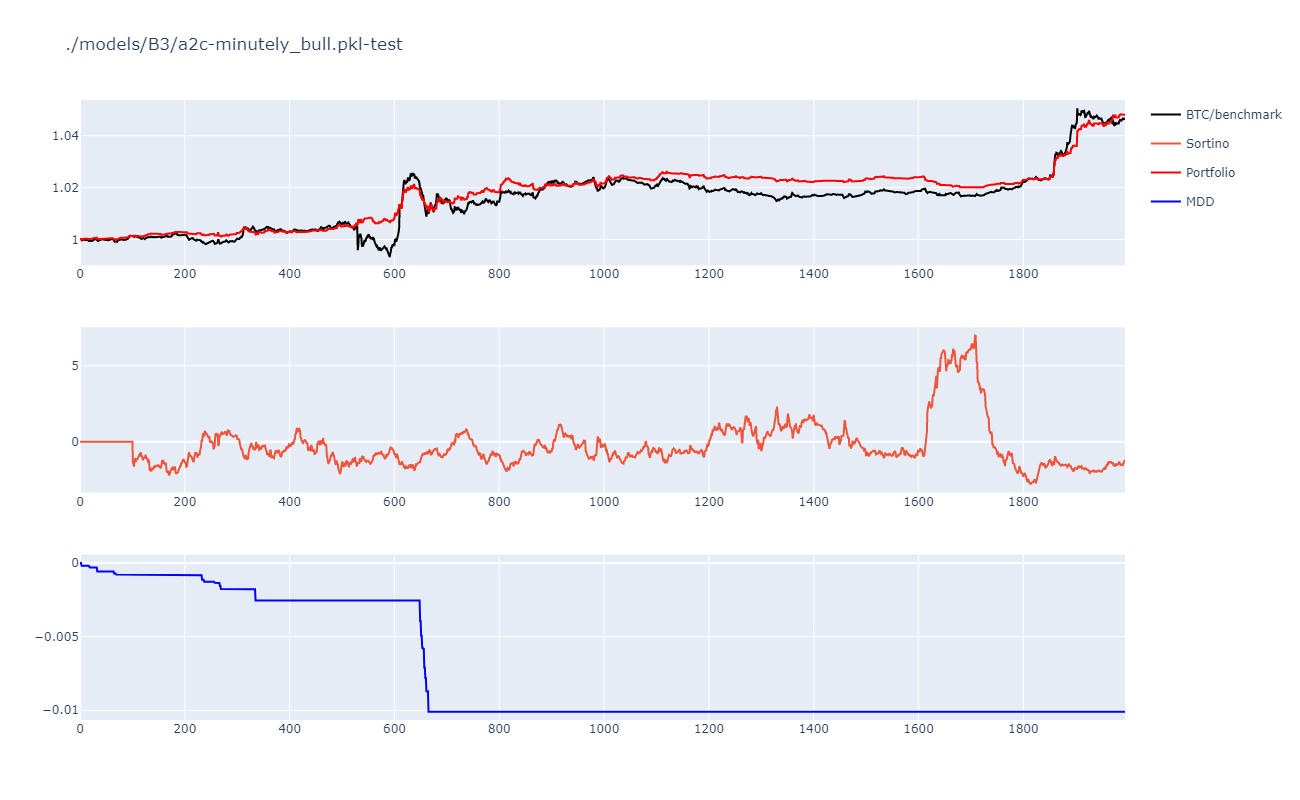
\includegraphics[width=0.94\textwidth]{graphics/testphoto/a2c-cont-mbu.png}
    \caption{Continuous A2C agent metrics for minute bull data}
    \label{f-a2c-cont-mbu}
\end{figure}

\subsection{PPO Strategy Agent (Discrete)}
This PPO agent is used with a discrete action space. The Discrete PPO agent performed weakly at the first 2 million timestamps, then surged after. Among 10 training runs, similar peaks appear and vanish in a similar way at random episodes. The representative model is taken from the final result of the training session shown in Fig. \ref{gr:ppod:train}, at timestamp 2,228,800 (200th episode, $\sim$5,000 seconds).

\begin{figure}[H]
    \centering
    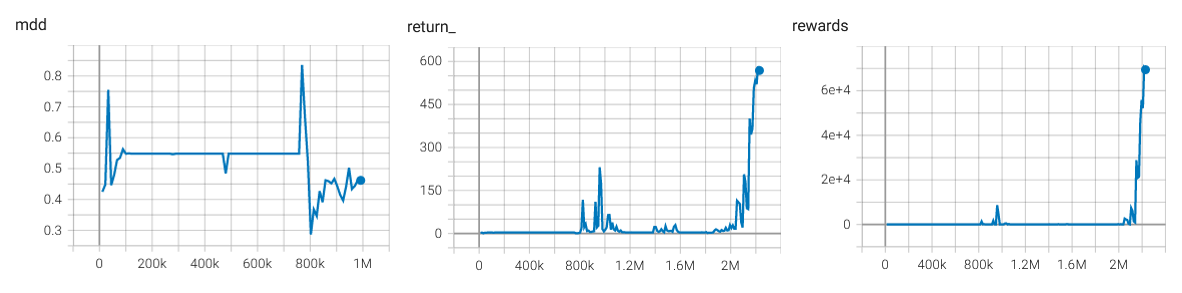
\includegraphics[width=0.99\textwidth]{graphics/trainphoto/ppodtrain.png}
    \caption{Discrete PPO Training Results}
    \label{gr:ppod:train}
\end{figure}

The model, scoring 600 at training return value, i.e., 59,900\% profit over the training data, results in a significant profit in \texttt{HBu} and \texttt{HBr} test datasets, performing in average 59.88\% and 153.96\% better than benchmark, respectively. However, the Discrete PPO agent is not much better than benchmark in minute test datasets. Overall, it performs better in all aspects (return, MDD) compared to the benchmark. See Table \ref{resl:disc-ppo}.

\begin{longtable}[c]{|l|rrr|rrr|r|c|}
\caption{Discrete PPO Test Results}
\label{resl:disc-ppo}\\
\hline
\multicolumn{1}{|c|}{\multirow{2}{*}{\textbf{$\mathcal{D}$}}} & \multicolumn{3}{c|}{\textbf{Agent}} & \multicolumn{3}{c|}{\textbf{Benchmark}} & \multicolumn{1}{c|}{\multirow{2}{*}{\textbf{$\overline{\Delta\phi_{\alpha,\odot}}$}}} & \multirow{2}{*}{\textbf{Fig.}} \\ \cline{2-7}
\multicolumn{1}{|c|}{} & \multicolumn{1}{c|}{\textbf{Return}} & \multicolumn{1}{c|}{\textbf{MDD}} & \multicolumn{1}{c|}{\textit{\textbf{Sortino}}} & \multicolumn{1}{c|}{\textbf{Return}} & \multicolumn{1}{c|}{\textbf{MDD}} & \multicolumn{1}{c|}{\textit{\textbf{Sortino}}} & \multicolumn{1}{c|}{} &  \\ \hline
\endfirsthead
%
\multicolumn{9}{c}%
{{\bfseries Table \thetable\ continued from previous page}} \\
\endhead
%
\textbf{\texttt{HBu}} & \multicolumn{1}{r|}{\textbf{1.6982}} & \multicolumn{1}{r|}{\textbf{0.0725}} & \textit{-1.1362} & \multicolumn{1}{r|}{0.2643} & \multicolumn{1}{r|}{0.1174} & \textit{0.7060} & 0.5988 & \ref{f-ppo-disc-hbu} \\ \hline
\textbf{\texttt{HBr}} & \multicolumn{1}{r|}{\textbf{2.2585}} & \multicolumn{1}{r|}{\textbf{0.1014}} & \textit{-3.2534} & \multicolumn{1}{r|}{-0.4484} & \multicolumn{1}{r|}{0.5199} & \textit{-0.3982} & 1.5396 & \ref{f-ppo-disc-hbr} \\ \hline
\textbf{\texttt{MCr}} & \multicolumn{1}{r|}{\textbf{0.0090}} & \multicolumn{1}{r|}{\textbf{0.0363}} & \textit{1.9876} & \multicolumn{1}{r|}{-0.0361} & \multicolumn{1}{r|}{0.0725} & \textit{-0.2276} & 0.0287 & \ref{f-ppo-disc-mcr} \\ \hline
\textbf{\texttt{MBu}} & \multicolumn{1}{r|}{\textbf{0.0475}} & \multicolumn{1}{r|}{\textbf{0.0146}} & \textit{-1.0178} & \multicolumn{1}{r|}{0.0441} & \multicolumn{1}{r|}{0.0164} & \textit{1.0024} & 0.0006 & \ref{f-ppo-disc-mbu} \\ \hline
\end{longtable}


\begin{figure}[H]
    \centering
    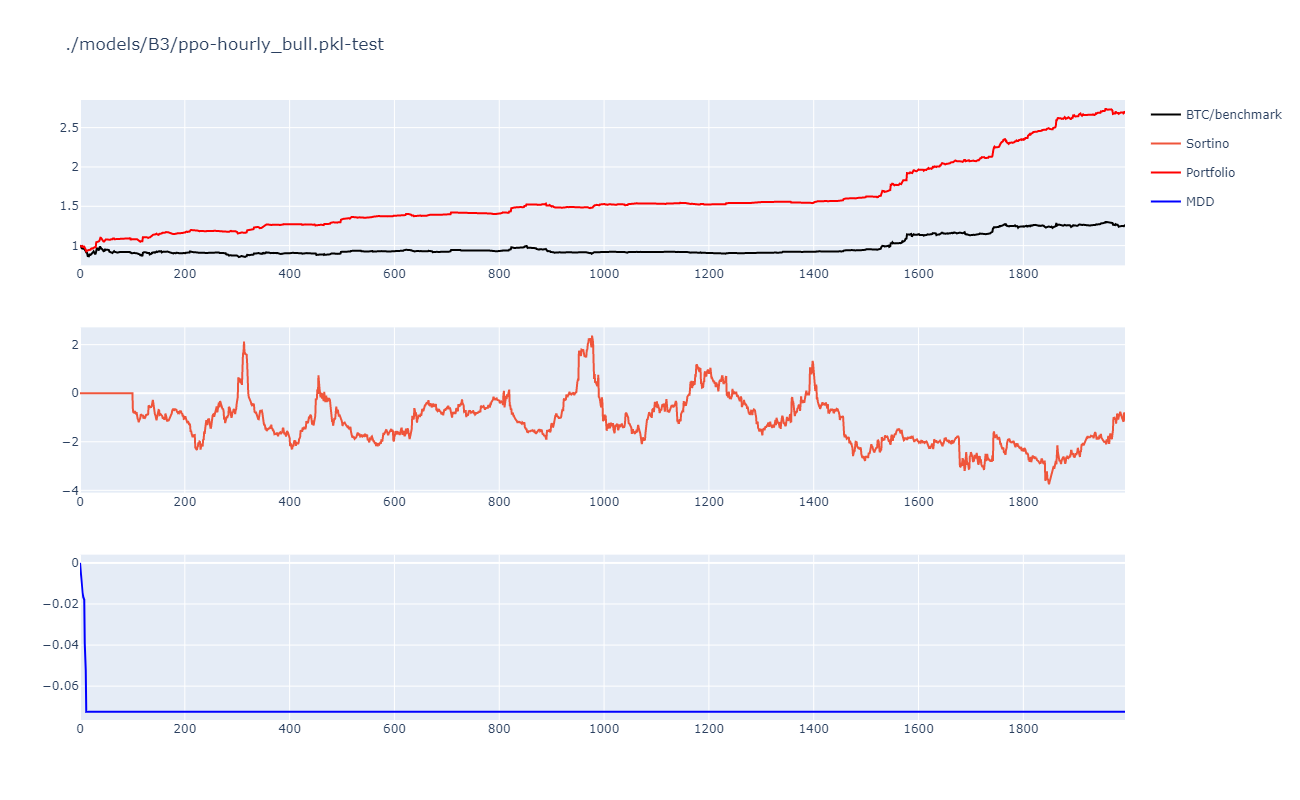
\includegraphics[width=0.94\textwidth]{graphics/testphoto/ppo-disc-hbu.png}
    \caption{Discrete PPO agent metrics for hourly bull data}
    \label{f-ppo-disc-hbu}
\end{figure}

\begin{figure}[H]
    \centering
    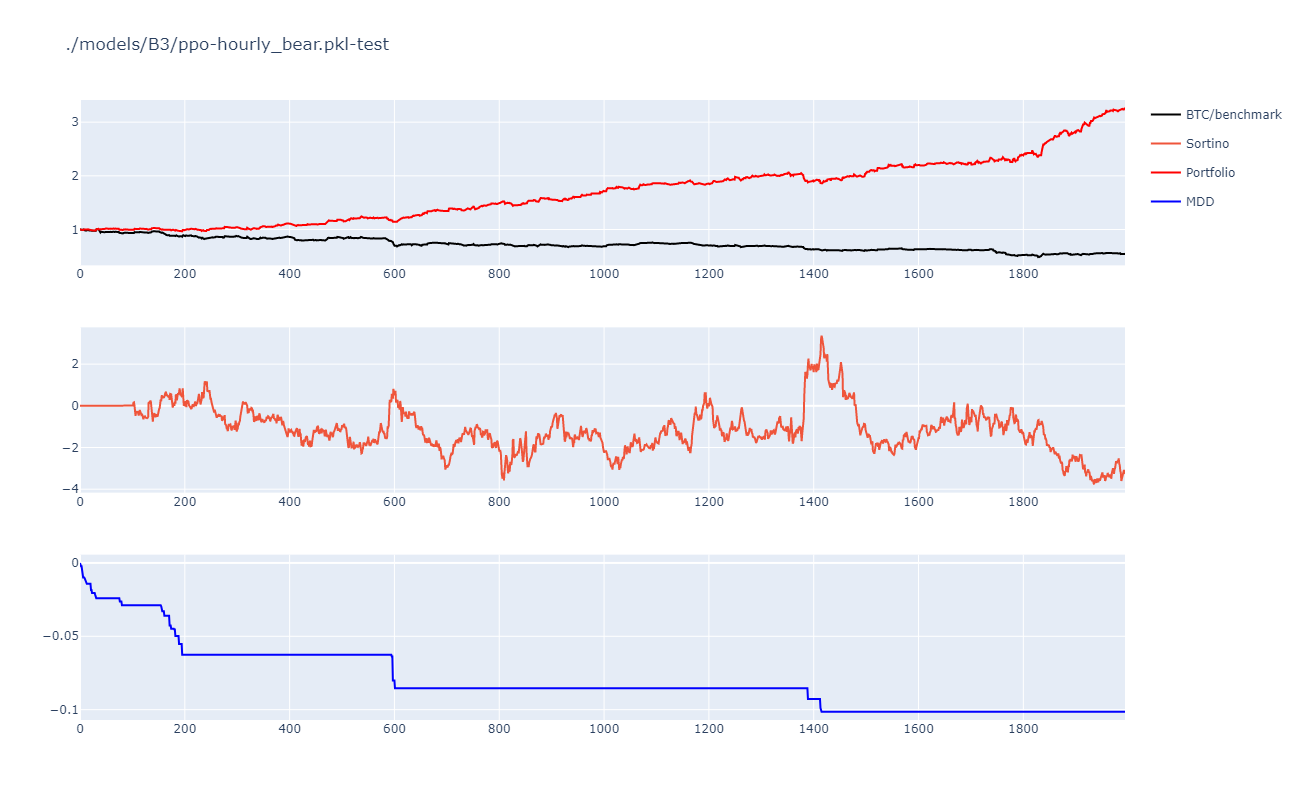
\includegraphics[width=0.94\textwidth]{graphics/testphoto/ppo-disc-hbr.png}
    \caption{Discrete PPO agent metrics for hourly bear data}
    \label{f-ppo-disc-hbr}
\end{figure}

\begin{figure}[H]
    \centering
    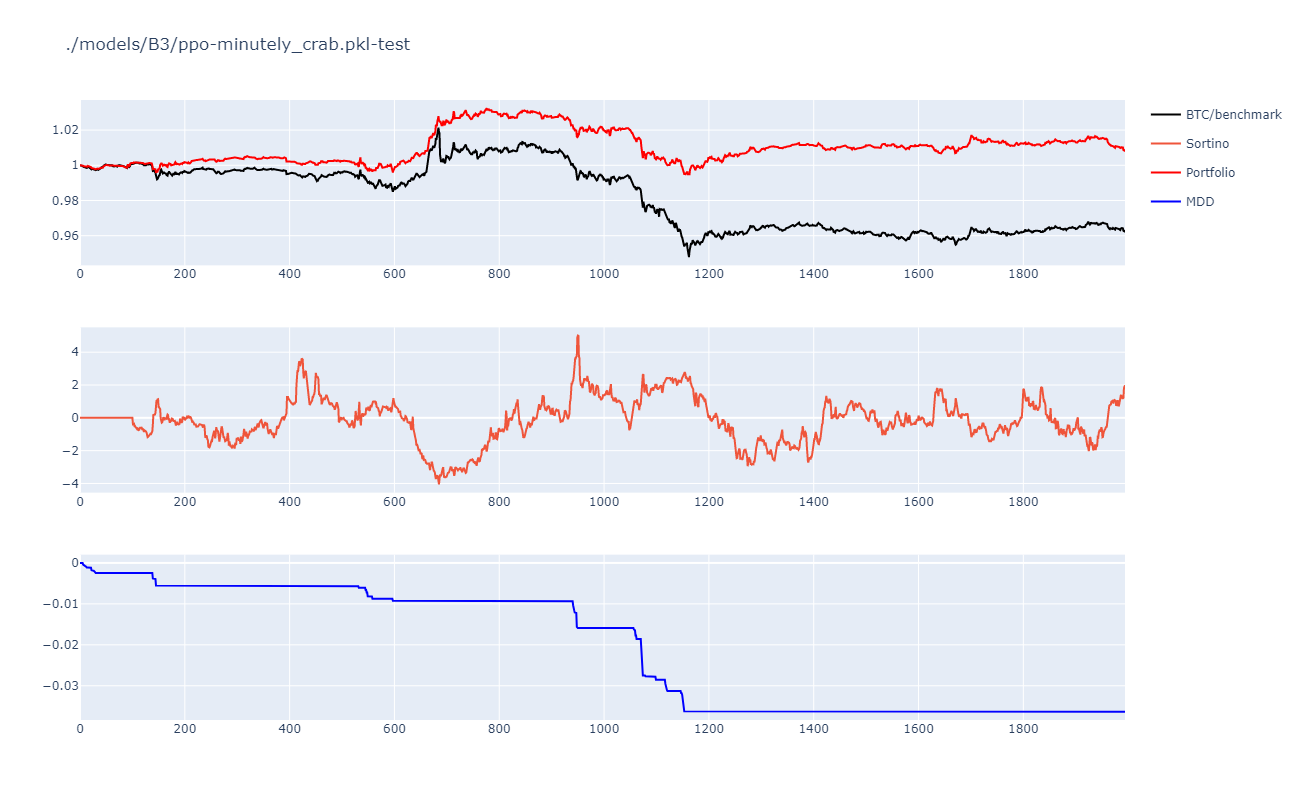
\includegraphics[width=0.94\textwidth]{graphics/testphoto/ppo-disc-mcr.png}
    \caption{Discrete PPO agent metrics for minute crab data}
    \label{f-ppo-disc-mcr}
\end{figure}

\begin{figure}[H]
    \centering
    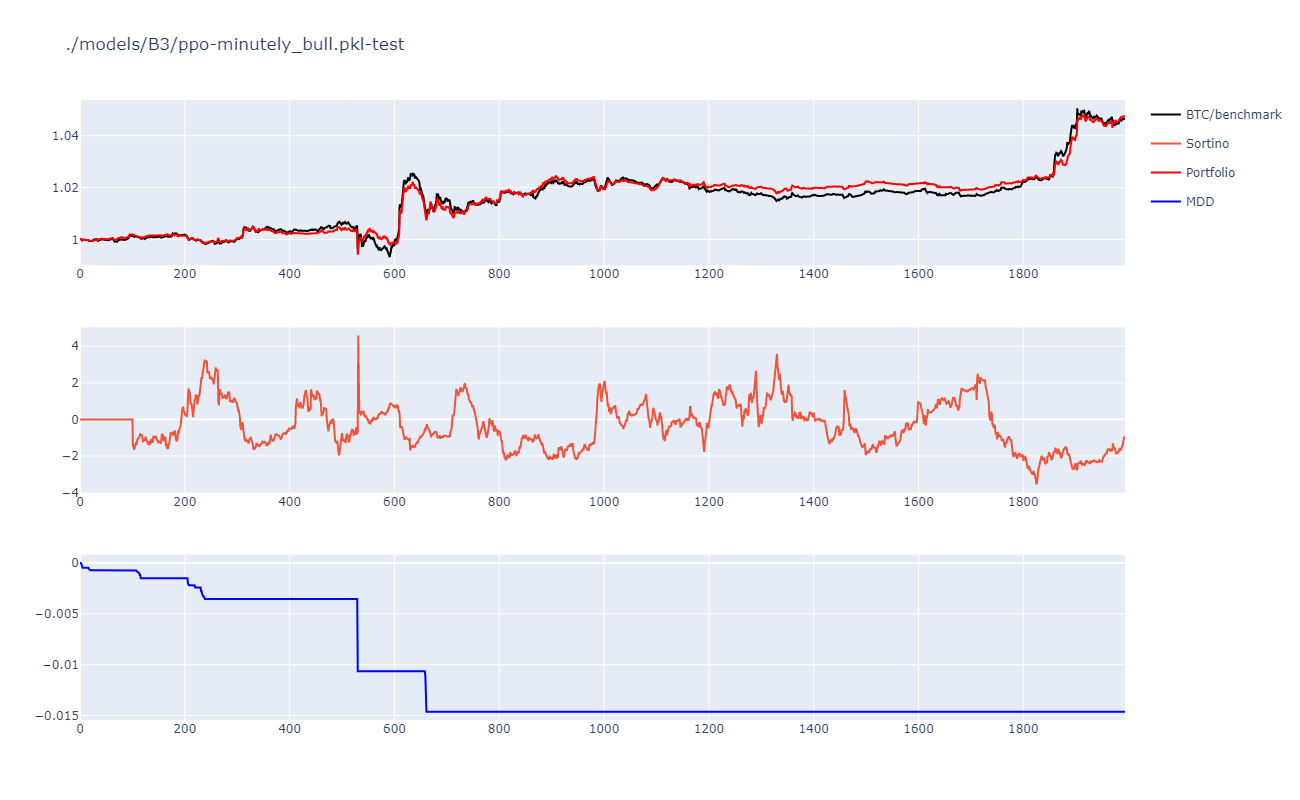
\includegraphics[width=0.94\textwidth]{graphics/testphoto/ppo-disc-mbu.png}
    \caption{Discrete PPO agent metrics for minute bull data}
    \label{f-ppo-disc-mbu}
\end{figure}

\subsection{PPO Strategy Agent (Continuous)}
This PPO agent is used with a continuous action space. The Continuous PPO agent results in more stable metrics over Discrete PPO, converging at around 1,800,000 timesteps ($\sim$167 episodes, $\sim$5,100 seconds) after having a peaking reward value at around 1,400,000 timesteps. Refer to Fig. \ref{gr:ppoc:train}.

\begin{figure}[H]
    \centering
    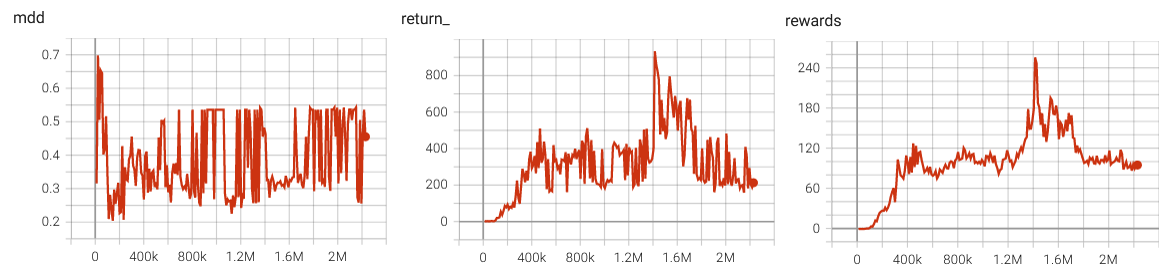
\includegraphics[width=0.99\textwidth]{graphics/trainphoto/ppoctrain.png}
    \caption{Continuous PPO Training Results}
    \label{gr:ppoc:train}
\end{figure}

Like Discrete PPO agent but less powerful, this Continuous PPO agent performs better than benchmark in all aspects, particularly the hourly datasets. An exception is the final return value for \texttt{MBu} dataset, where it performs 5.6\% lower than benchmark. See Table \ref{resl:cont-ppo}.

\begin{longtable}[c]{|l|rrr|rrr|r|c|}
\caption{Continuous PPO Test Results}
\label{resl:cont-ppo}\\
\hline
\multicolumn{1}{|c|}{\multirow{2}{*}{\textbf{$\mathcal{D}$}}} & \multicolumn{3}{c|}{\textbf{Agent}} & \multicolumn{3}{c|}{\textbf{Benchmark}} & \multicolumn{1}{c|}{\multirow{2}{*}{\textbf{$\overline{\Delta\phi_{\alpha,\odot}}$}}} & \multirow{2}{*}{\textbf{Fig.}} \\ \cline{2-7}
\multicolumn{1}{|c|}{} & \multicolumn{1}{c|}{\textbf{Return}} & \multicolumn{1}{c|}{\textbf{MDD}} & \multicolumn{1}{c|}{\textit{\textbf{Sortino}}} & \multicolumn{1}{c|}{\textbf{Return}} & \multicolumn{1}{c|}{\textbf{MDD}} & \multicolumn{1}{c|}{\textit{\textbf{Sortino}}} & \multicolumn{1}{c|}{} &  \\ \hline
\endfirsthead
%
\multicolumn{9}{c}%
{{\bfseries Table \thetable\ continued from previous page}} \\
\endhead
%
\textbf{\texttt{HBu}} & \multicolumn{1}{r|}{\textbf{0.6357}} & \multicolumn{1}{r|}{\textbf{0.0718}} & \textit{-1.2784} & \multicolumn{1}{r|}{0.2643} & \multicolumn{1}{r|}{0.1174} & \textit{0.7060} & 0.1897 & \ref{f-ppo-cont-hbu} \\ \hline
\textbf{\texttt{HBr}} & \multicolumn{1}{r|}{\textbf{0.2589}} & \multicolumn{1}{r|}{\textbf{0.1766}} & \textit{-1.6469} & \multicolumn{1}{r|}{-0.4484} & \multicolumn{1}{r|}{0.5199} & \textit{-0.3982} & 0.5571 & \ref{f-ppo-cont-hbr} \\ \hline
\textbf{\texttt{MCr}} & \multicolumn{1}{r|}{\textbf{-0.0265}} & \multicolumn{1}{r|}{\textbf{0.0551}} & \textit{2.0327} & \multicolumn{1}{r|}{-0.0361} & \multicolumn{1}{r|}{0.0725} & \textit{-0.2276} & 0.0057 & \ref{f-ppo-cont-mcr} \\ \hline
\textbf{\texttt{MBu}} & \multicolumn{1}{r|}{0.0416} & \multicolumn{1}{r|}{\textbf{0.0118}} & \textit{-0.0144} & \multicolumn{1}{r|}{\textbf{0.0441}} & \multicolumn{1}{r|}{0.0164} & \textit{1.0024} & 0.0017 & \ref{f-ppo-cont-mbu} \\ \hline
\end{longtable}


\begin{figure}[H]
    \centering
    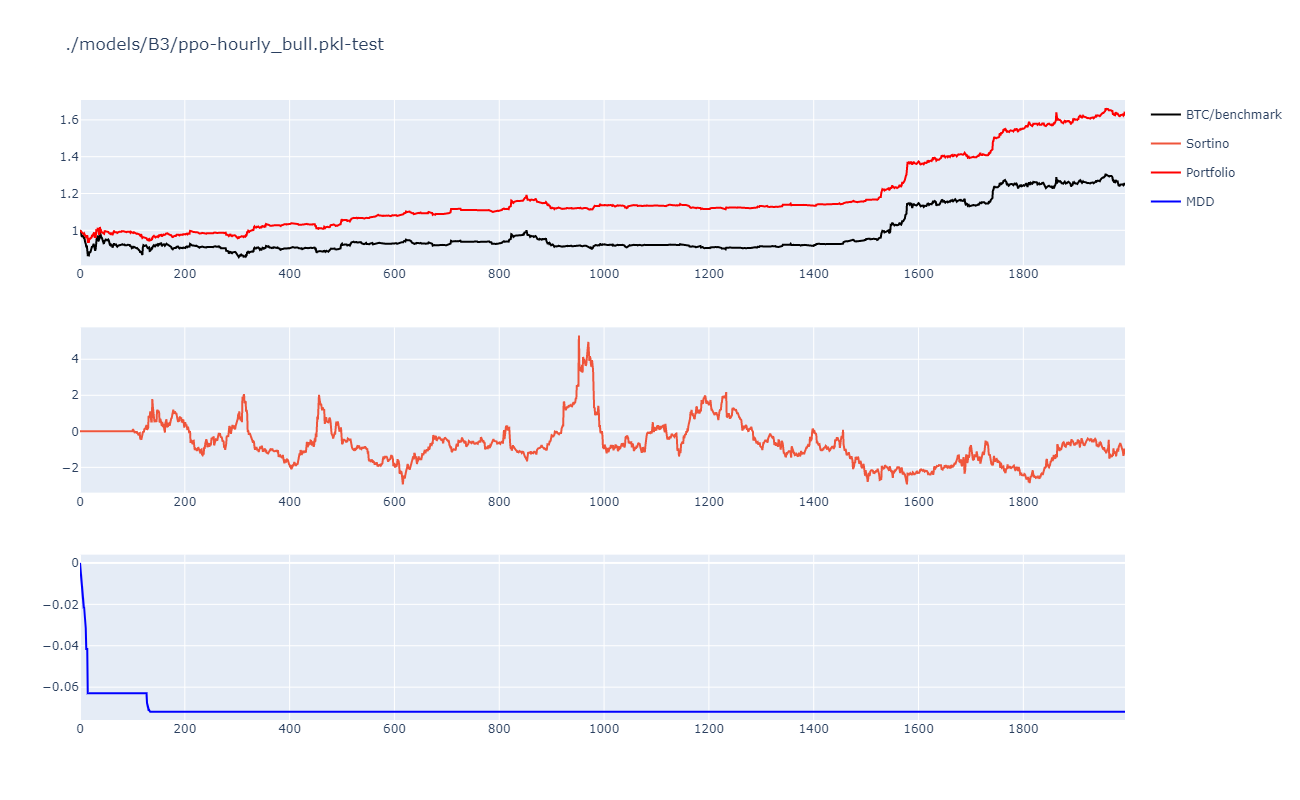
\includegraphics[width=0.94\textwidth]{graphics/testphoto/ppo-cont-hbu.png}
    \caption{Continuous PPO agent metrics for hourly bull data}
    \label{f-ppo-cont-hbu}
\end{figure}

\begin{figure}[H]
    \centering
    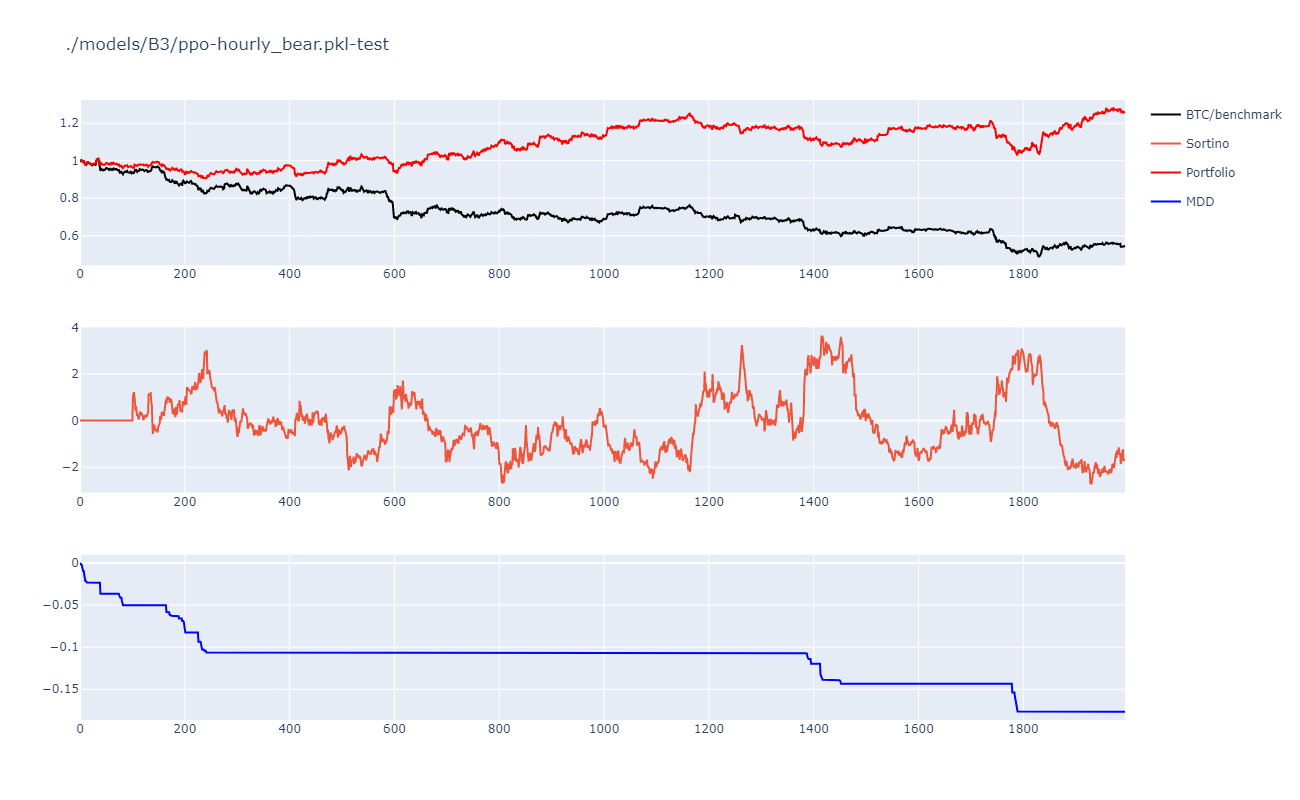
\includegraphics[width=0.94\textwidth]{graphics/testphoto/ppo-cont-hbr.png}
    \caption{Continuous PPO agent metrics for hourly bear data}
    \label{f-ppo-cont-hbr}
\end{figure}

\begin{figure}[H]
    \centering
    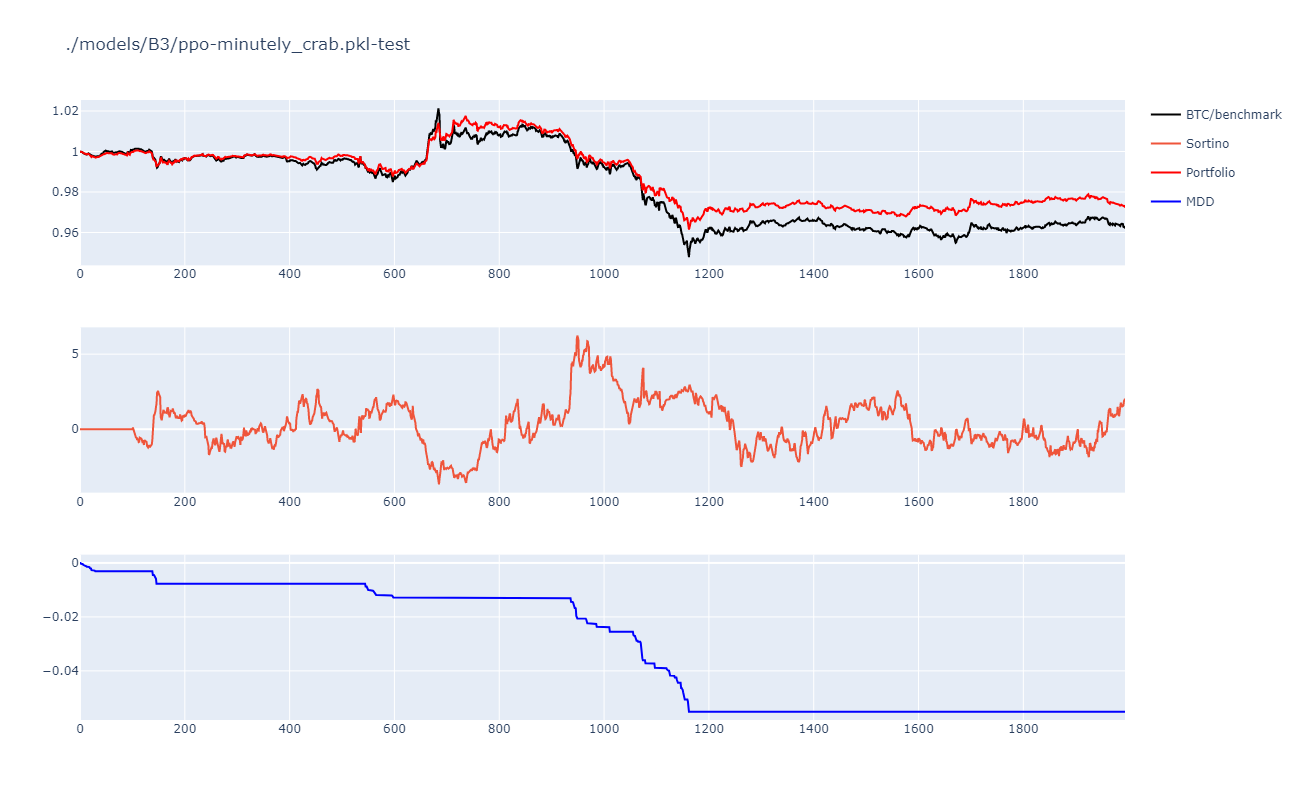
\includegraphics[width=0.94\textwidth]{graphics/testphoto/ppo-cont-mcr.png}
    \caption{Continuous PPO agent metrics for minute crab data}
    \label{f-ppo-cont-mcr}
\end{figure}

\begin{figure}[H]
    \centering
    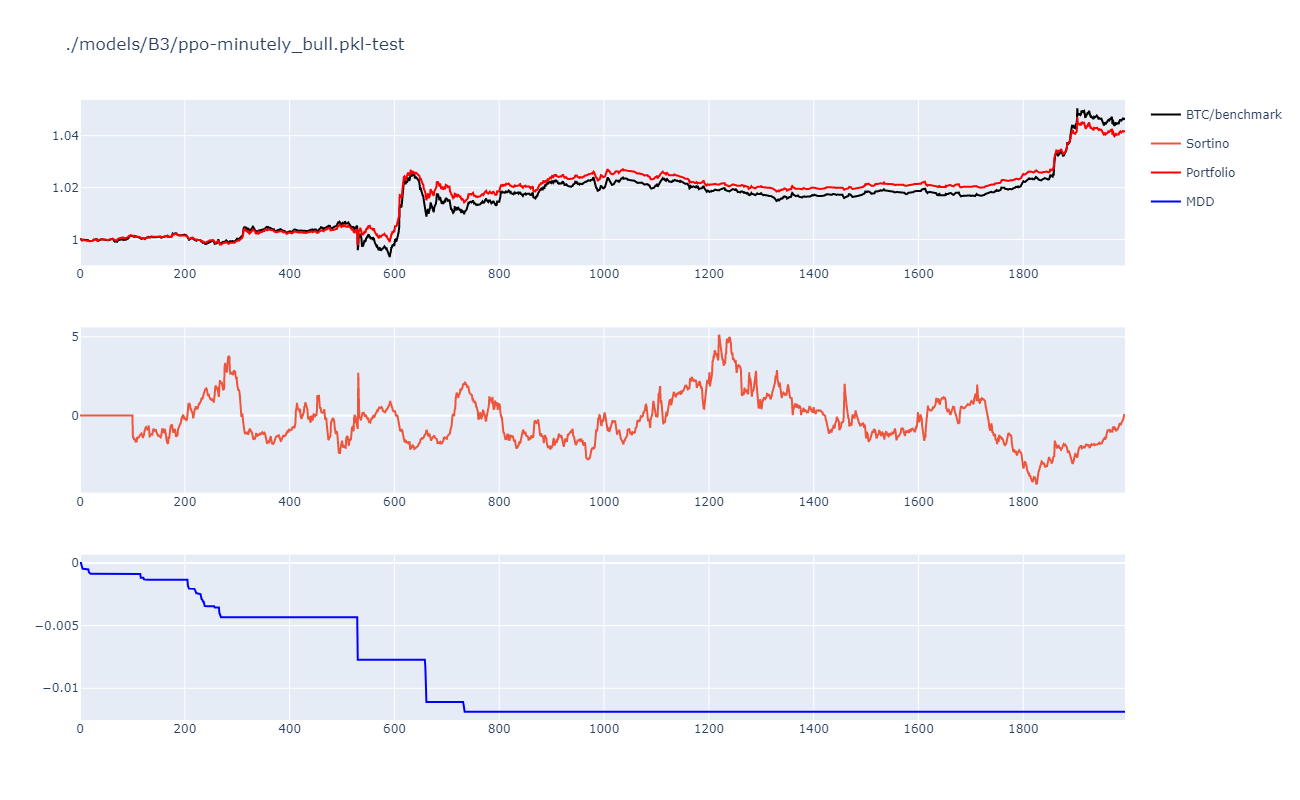
\includegraphics[width=0.94\textwidth]{graphics/testphoto/ppo-cont-mbu.png}
    \caption{Continuous PPO agent metrics for minute bull data}
    \label{f-ppo-cont-mbu}
\end{figure}

\subsection{SAC Strategy Agent (Continuous)}
The SAC agent operates in the continuous action space. Unlike the other agents, the SAC agent takes approximately 10 times more training duration to complete one episode. Using early stopping, the representative model is taken from timestamp 1,080,968 (97th episode, $\sim$25,800 seconds). Refer to Fig. \ref{gr:sac:train}.

\begin{figure}[H]
    \centering
    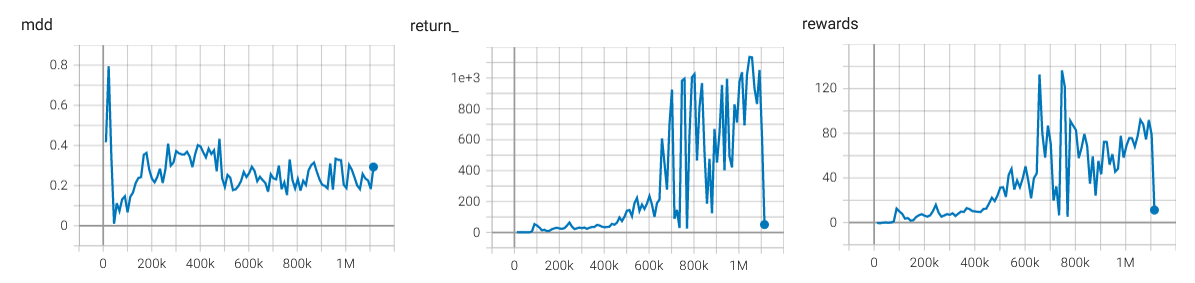
\includegraphics[width=0.99\textwidth]{graphics/trainphoto/sac-train.png}
    \caption{SAC Training Results}
    \label{gr:sac:train}
\end{figure}

Despite the high reward and return values, on top of its longer training duration, the SAC agent performs similarly to the Continuous PPO agent, yet less satisfying. The SAC agent averages around 10–13\% higher than benchmark in hourly data, but rather equal to benchmark in minute data. However, this agent successfully dampens the maximum drawdown in all cases. See Table \ref{resl:-sac}.

\begin{longtable}[c]{|l|rrr|rrr|r|c|}
\caption{SAC Test Results}
\label{resl:-sac}\\
\hline
\multicolumn{1}{|c|}{\multirow{2}{*}{\textbf{$\mathcal{D}$}}} & \multicolumn{3}{c|}{\textbf{Agent}} & \multicolumn{3}{c|}{\textbf{Benchmark}} & \multicolumn{1}{c|}{\multirow{2}{*}{\textbf{$\overline{\Delta\phi_{\alpha,\odot}}$}}} & \multirow{2}{*}{\textbf{Fig.}} \\ \cline{2-7}
\multicolumn{1}{|c|}{} & \multicolumn{1}{c|}{\textbf{Return}} & \multicolumn{1}{c|}{\textbf{MDD}} & \multicolumn{1}{c|}{\textit{\textbf{Sortino}}} & \multicolumn{1}{c|}{\textbf{Return}} & \multicolumn{1}{c|}{\textbf{MDD}} & \multicolumn{1}{c|}{\textit{\textbf{Sortino}}} & \multicolumn{1}{c|}{} &  \\ \hline
\endfirsthead
%
\multicolumn{9}{c}%
{{\bfseries Table \thetable\ continued from previous page}} \\
\endhead
%
\textbf{\texttt{HBu}} & \multicolumn{1}{r|}{\textbf{0.3782}} & \multicolumn{1}{r|}{\textbf{0.0879}} & \textit{-1.1721} & \multicolumn{1}{r|}{0.2643} & \multicolumn{1}{r|}{0.1174} & \textit{0.7060} & 0.1097 & \ref{f-sac-hbu} \\ \hline
\textbf{\texttt{HBr}} & \multicolumn{1}{r|}{\textbf{-0.1993}} & \multicolumn{1}{r|}{\textbf{0.2915}} & \textit{-0.6846} & \multicolumn{1}{r|}{-0.4484} & \multicolumn{1}{r|}{0.5199} & \textit{-0.3982} & 0.1361 & \ref{f-sac-hbr} \\ \hline
\textbf{\texttt{MCr}} & \multicolumn{1}{r|}{\textbf{-0.0295}} & \multicolumn{1}{r|}{\textbf{0.0439}} & \textit{1.5296} & \multicolumn{1}{r|}{-0.0361} & \multicolumn{1}{r|}{0.0725} & \textit{-0.2276} & 0.0030 & \ref{f-sac-mcr} \\ \hline
\textbf{\texttt{MBu}} & \multicolumn{1}{r|}{0.0222} & \multicolumn{1}{r|}{\textbf{0.0105}} & \textit{-0.6082} & \multicolumn{1}{r|}{\textbf{0.0441}} & \multicolumn{1}{r|}{0.0164} & \textit{1.0024} & -0.0065 & \ref{f-sac-mbu} \\ \hline
\end{longtable}

\begin{figure}[H]
    \centering
    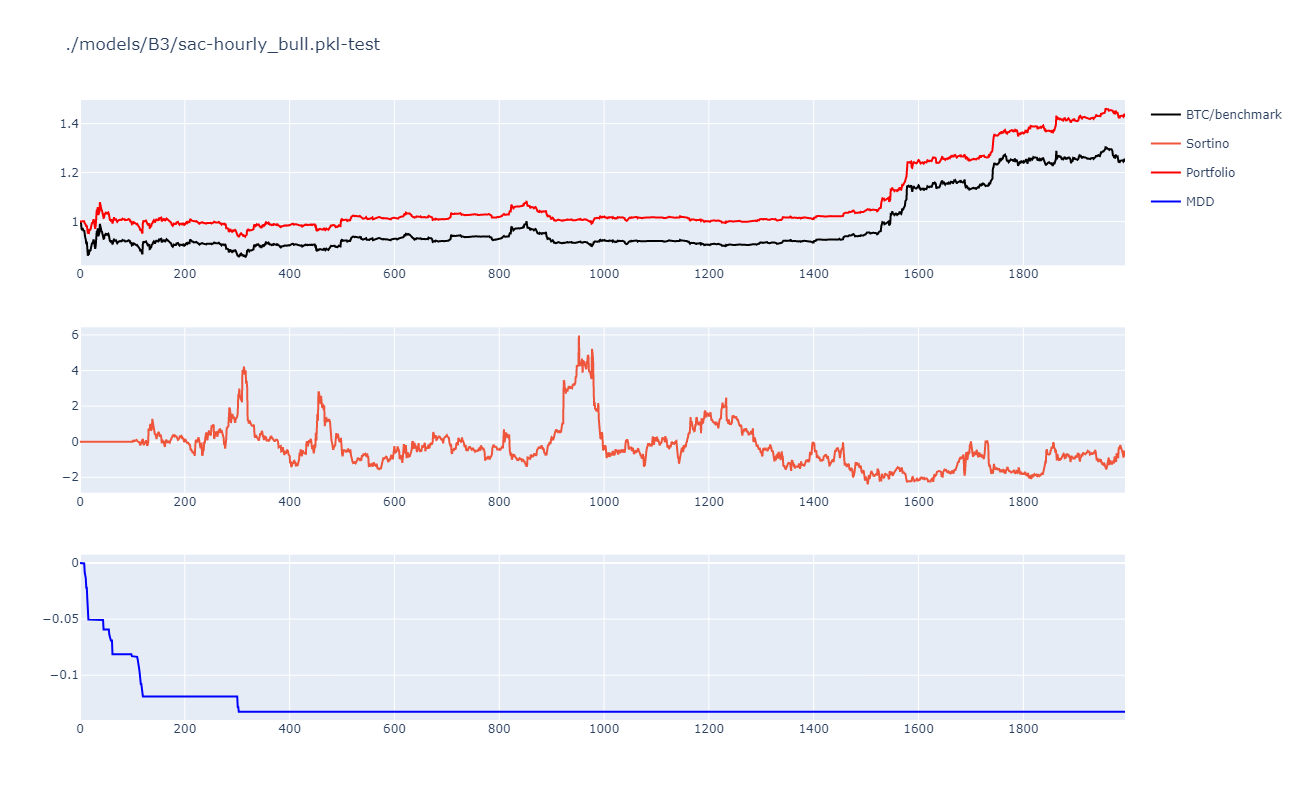
\includegraphics[width=0.94\textwidth]{graphics/testphoto/sac-hbu.png}
    \caption{SAC agent metrics for hourly bull data}
    \label{f-sac-hbu}
\end{figure}

\begin{figure}[H]
    \centering
    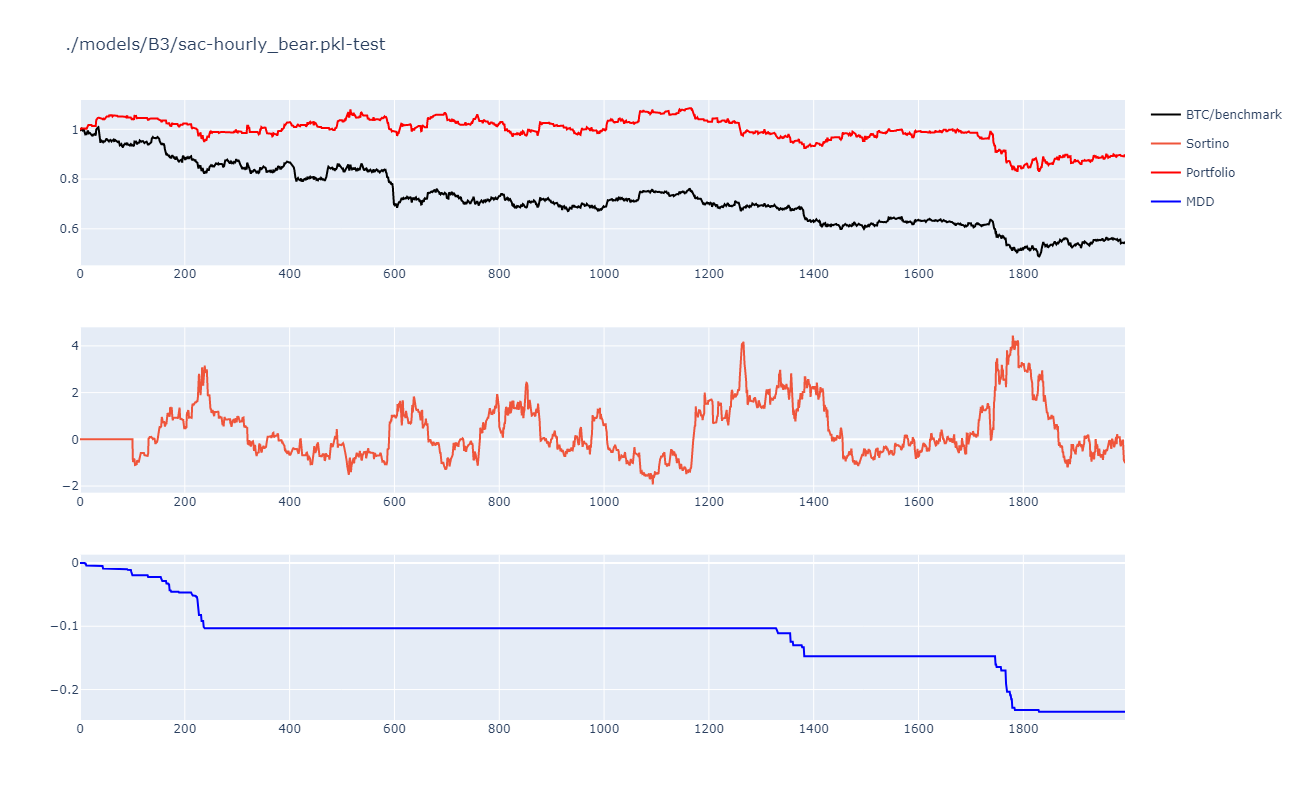
\includegraphics[width=0.94\textwidth]{graphics/testphoto/sac-hbr.png}
    \caption{SAC agent metrics for hourly bear data}
    \label{f-sac-hbr}
\end{figure}

\begin{figure}[H]
    \centering
    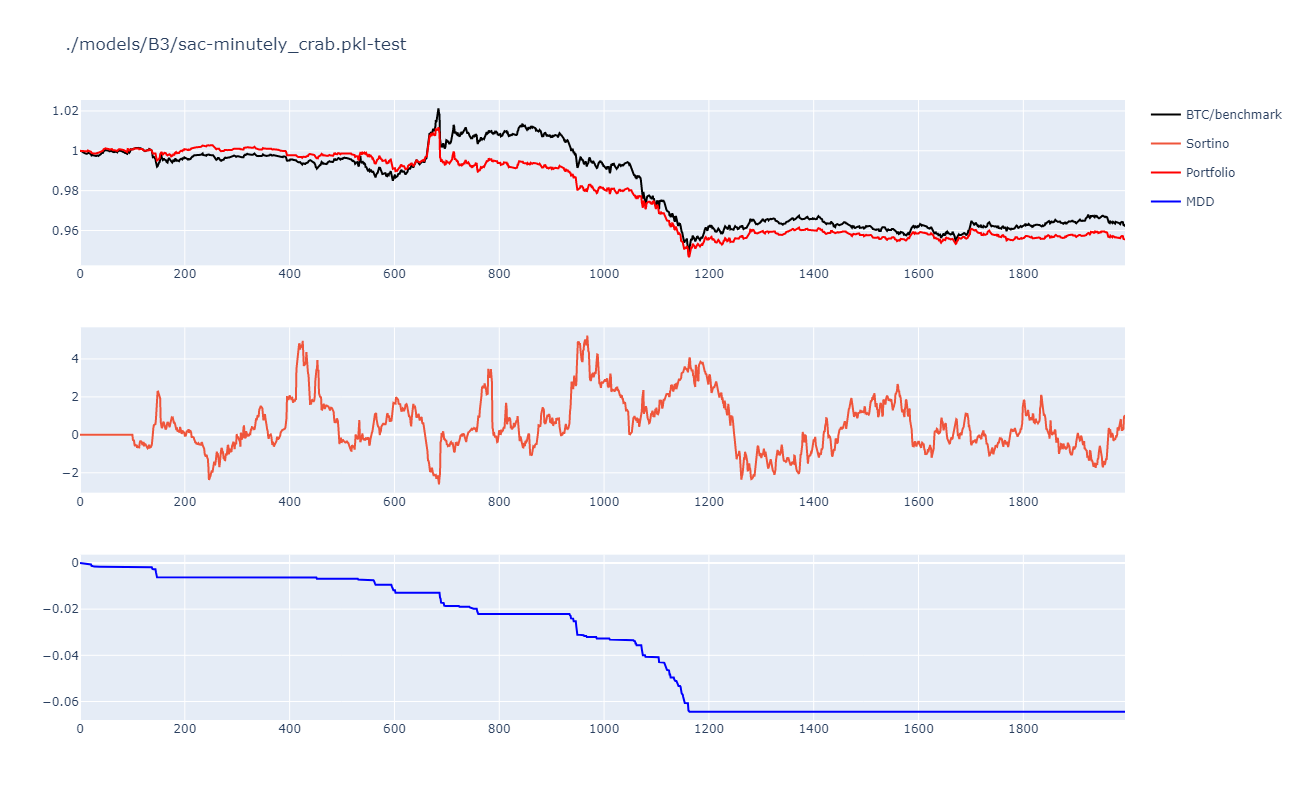
\includegraphics[width=0.94\textwidth]{graphics/testphoto/sac-mcr.png}
    \caption{SAC agent metrics for minute crab data}
    \label{f-sac-mcr}
\end{figure}

\begin{figure}[H]
    \centering
    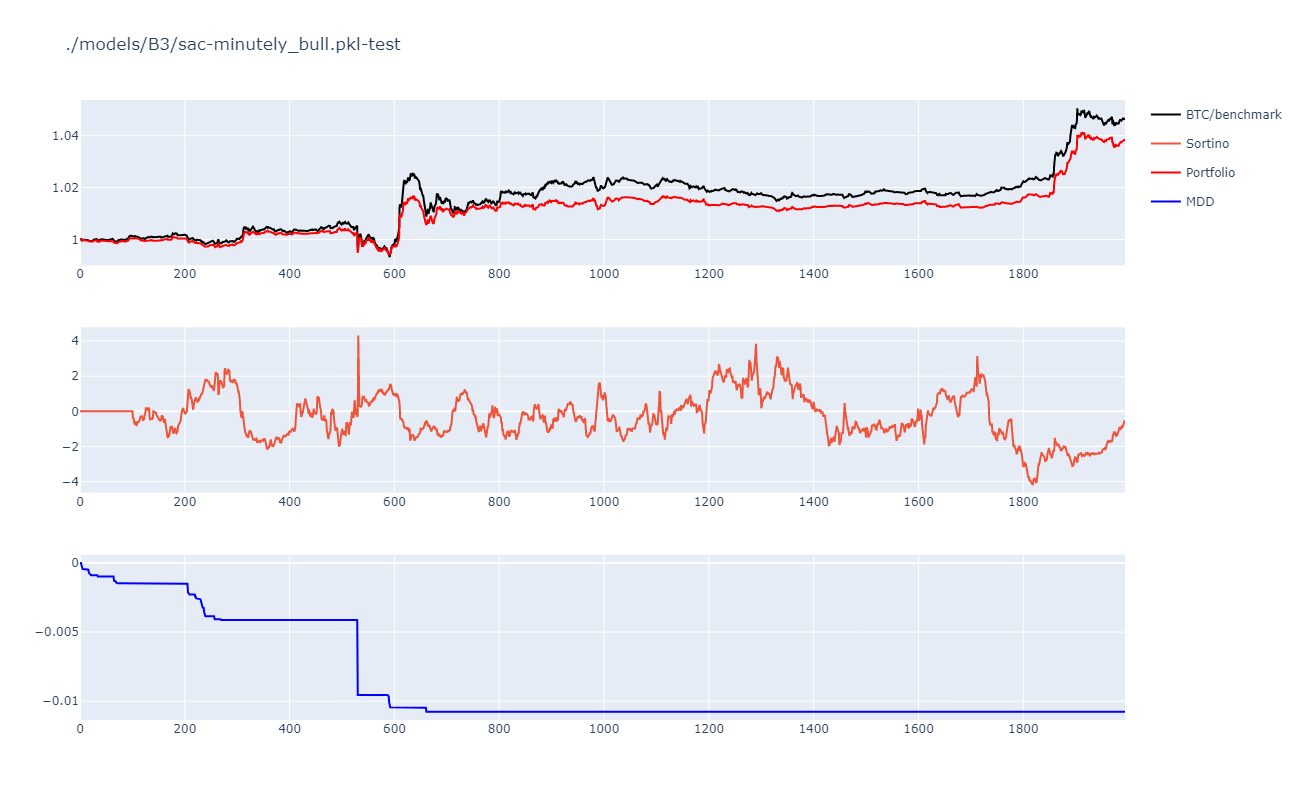
\includegraphics[width=0.94\textwidth]{graphics/testphoto/sac-mbu.png}
    \caption{SAC agent metrics for minute bull data}
    \label{f-sac-mbu}
\end{figure}

